\documentclass[12pt, a4paper]{article}
\usepackage[utf8]{inputenc}
\usepackage[T1]{fontenc}
\usepackage{ngerman}
\usepackage{amsmath, amssymb, amsthm}
\usepackage{mathtools}
\usepackage{bm}
\usepackage{graphicx}
\usepackage{xcolor}
\usepackage{pgfplots}
\pgfplotsset{compat=1.18}
\usepackage{tikz}
\usetikzlibrary{arrows.meta, positioning, shapes.geometric, calc,
                decorations.pathreplacing, matrix, fit, backgrounds}
\usepackage{booktabs}
\usepackage{array}
\usepackage{longtable}
\usepackage{geometry}
\usepackage{setspace}
\usepackage{parskip}
\usepackage{hyperref}
\usepackage{cleveref}
\usepackage{natbib}
\usepackage{caption}
\usepackage{subcaption}
\usepackage{algorithm}
\usepackage{algpseudocode}
\usepackage{enumitem}
\usepackage{multirow}
\usepackage{float}
\usepackage{rotating}
\usepackage{microtype}
\setlist[itemize,1]{label=--}

\geometry{margin=2.5cm}

% ---------- Farben ----------
\definecolor{mainblue}{RGB}{25, 70, 140}
\definecolor{accentred}{RGB}{180, 50, 30}
\definecolor{lightgray}{RGB}{245, 245, 248}
\definecolor{darkgray}{RGB}{60, 60, 70}
\definecolor{darkgreen}{RGB}{30, 100, 50}
\definecolor{darkorange}{RGB}{200, 100, 0}

% ---------- Theorem-Umgebungen ----------
\newtheorem{theorem}{Theorem}[section]
\newtheorem{lemma}[theorem]{Lemma}
\newtheorem{proposition}[theorem]{Proposition}
\newtheorem{corollary}[theorem]{Korollar}
\theoremstyle{definition}
\newtheorem{definition}[theorem]{Definition}
\newtheorem{example}[theorem]{Beispiel}
\theoremstyle{remark}
\newtheorem{remark}[theorem]{Bemerkung}

% ---------- Hyperref ----------
\hypersetup{
  colorlinks=true,
  linkcolor=mainblue,
  citecolor=accentred,
  urlcolor=mainblue,
  pdftitle={Die Matrix als maximal kompakte mathematische Darstellung},
  pdfauthor={Stephan Epp},
}

% ---------- Makros ----------
\newcommand{\R}{\mathbb{R}}
\newcommand{\C}{\mathbb{C}}
\newcommand{\N}{\mathbb{N}}
\newcommand{\Z}{\mathbb{Z}}
\newcommand{\vx}{\bm{x}}
\newcommand{\vu}{\bm{u}}
\newcommand{\vy}{\bm{y}}
\newcommand{\vA}{\bm{A}}
\newcommand{\vB}{\bm{B}}
\newcommand{\vC}{\bm{C}}
\newcommand{\vP}{\bm{P}}
\newcommand{\vQ}{\bm{Q}}
\newcommand{\vI}{\bm{I}}
\newcommand{\vV}{\bm{V}}
\newcommand{\vLambda}{\bm{\Lambda}}
\newcommand{\vK}{\bm{K}}
\newcommand{\vR}{\bm{R}}
\newcommand{\vG}{\bm{G}}
\newcommand{\vS}{\bm{S}}
\newcommand{\vSigma}{\bm{\Sigma}}
\newcommand{\vD}{\bm{D}}
\newcommand{\vL}{\bm{L}}
\newcommand{\vT}{\bm{T}}
\newcommand{\T}{\top}
\newcommand{\tr}{\mathrm{tr}}
\newcommand{\rank}{\mathrm{rank}}
\newcommand{\spec}{\sigma}
\newcommand{\re}{\mathrm{Re}}
\newcommand{\im}{\mathrm{Im}}
\newcommand{\diag}{\mathrm{diag}}

\title{\textbf{Die Matrix als maximal kompakte\\ mathematische Darstellung}\\[0.5em]
  {\Large\itshape Relationale Kapazität, Adjazenzisomorphie,\\ Spektraltheorie und universelle
   Darstellungskraft}}
\author{Stephan Epp}
\date{16. April 2026}

% ============================================================
\begin{document}
% ============================================================

\maketitle
\tableofcontents
\newpage

% ============================================================
\section{Einleitung}
\label{sec:einleitung}
% ============================================================

Die Matrix ist die schönste und kompakteste Schreibweise zur Beschreibung
mathematischer Strukturen und ihrer Beziehungen untereinander~\citep{horn2013}.
Diese Beobachtung, die auf den ersten Blick als ästhetisches Urteil erscheint,
lässt sich präzise mathematisch formalisieren und quantitativ belegen. Die
vorliegende Arbeit widmet sich genau dieser Frage: In welchem Sinne ist die
Matrix die kompakteste Darstellung, und was bedeutet Kompaktheit hier?

Die zentrale These lautet: Eine quadratische Matrix $\vA \in \R^{n \times n}$
realisiert in einer einzigen strukturierten Datenanordnung \emph{maximal viele
Beziehungen} zwischen $n$ Elementen -- nämlich genau $n^2$ Einträge, also
quadratisch viele. Keine andere elementare mathematische Struktur über einer
$n$-elementigen Grundmenge erreicht diese Dichte gleichzeitig bei voller
algebraischer Zugänglichkeit.

Im Vergleich dazu realisiert eine einfache mathematische Abbildung
$f: A \to B$ mit $|A| = |B| = n$ lediglich $n$ Zuordnungen -- linear viele.
Selbst ein vollständiger gerichteter Graph (Turniergraph) ohne Schleifen
kommt nur auf $n(n-1)$ Kanten, also $n^2 - n$ Beziehungen; die Matrix
ergänzt diese um genau $n$ Diagonaleinträge, die Selbstrelationen kodieren.

Die entscheidende und tief liegende zweite Aussage ist die Verbindung zur
Graphentheorie: Jede quadratische Matrix $\vA \in \R^{n \times n}$ induziert
\emph{kanonisch} einen gewichteten gerichteten Graphen $\mathcal{G}(\vA)$
über die Adjazenzmatrix-Konstruktion. Diese Bijektivität zwischen Matrizen
und gewichteten Digraphen ist nicht bloß eine Analogie -- sie ist eine exakte
mathematische Isomorphie, die sämtliche Algorithmen der Graphentheorie direkt
auf Matrizen übertragbar macht. Insbesondere der Subgraph Algorithmus
\citep{epp2026subgraph} und seine Werkzeuge der Tiefensuche, Breitensuche,
SCC-Zerlegung und Signaturkodierung sind somit unmittelbar als
Matrizenanalysemethoden einsetzbar~\citep{epp2026sysstate}.

\subsection{Wissenschaftliche Einordnung}
\label{subsec:einordnung}

Die vorliegende Arbeit verbindet drei Themenkomplexe:

\begin{enumerate}[label=(\roman*)]
  \item \textbf{Relationale Kapazität:} Formaler Nachweis, dass die quadratische
    Matrix unter allen elementaren mathematischen Darstellungen über $n$
    Elementen die höchste relationale Kapazität besitzt.

  \item \textbf{Adjazenzisomorphie:} Formaler Nachweis der Äquivalenz
    $\vA \leftrightarrow \mathcal{G}(\vA)$ und ihrer Konsequenzen für die
    Algorithmenübertragung.

  \item \textbf{Universelle Darstellungskraft:} Analyse, wie nahezu alle
    Kernbereiche der Mathematik -- Systemtheorie, Graphentheorie, Numerik,
    Statistik, Quantenmechanik, Netzwerktheorie -- die Matrix als
    fundamentale Sprache nutzen.
\end{enumerate}

\subsection{Aufbau der Arbeit}
\label{subsec:aufbau}

Abschnitt~\ref{sec:grundlagen} legt die mengentheoretischen Grundlagen der
relationalen Kapazität. Abschnitt~\ref{sec:kompaktheit} beweist den
Hauptsatz der maximalen Kompaktheit. Abschnitt~\ref{sec:adjazenz} behandelt
die Adjazenzisomorphie vollständig. Abschnitt~\ref{sec:spektral} entwickelt
die spektralen Eigenschaften. Abschnitt~\ref{sec:anwendungen} zeigt die
universelle Darstellungskraft. Abschnitt~\ref{sec:plots} beschreibt und
kommentiert alle erzeugten Abbildungen. Abschnitt~\ref{sec:ausblick} enthält
einen sehr ausführlichen Ausblick.

% ============================================================
\section{Mathematische Grundlagen}
\label{sec:grundlagen}
% ============================================================

\subsection{Mengen und Relationen}
\label{subsec:mengen}

\begin{definition}[Binäre Relation]
Seien $X$ und $Y$ nichtleere Mengen. Eine \emph{binäre Relation} von $X$
nach $Y$ ist eine Teilmenge $R \subseteq X \times Y$.
\end{definition}

\begin{definition}[Relationale Kapazität]
\label{def:rel_kap}
Die \emph{relationale Kapazität} einer mathematischen Struktur $\mathcal{S}$
über einer $n$-elementigen Grundmenge ist die maximale Anzahl
\[
  \kappa(\mathcal{S}) = \max\bigl|R\bigr|,
\]
wobei das Maximum über alle zulässigen Relationen $R$ der Struktur genommen wird.
\end{definition}

\begin{definition}[Abbildung, Graph, Matrix]
\label{def:drei}
Sei $X$ eine Menge mit $|X| = n$.
\begin{enumerate}[label=(\alph*)]
  \item Eine \emph{Abbildung} $f: X \to X$ ist eine Relation
    $R_f \subseteq X \times X$ mit $|R_f| = n$
    (genau ein Bild je Urbildelement).
  \item Ein \emph{gerichteter Graph} $G = (X, E)$ ist eine Relation
    $E \subseteq X \times X$, wobei $|E| \leq n(n-1)$ für schlingenfreie
    Graphen gilt.
  \item Eine \emph{quadratische Matrix} $\vA \in \R^{n \times n}$ ist eine
    Abbildung $\vA: \{1,\ldots,n\}^2 \to \R$, die $n^2$ reelle Werte
    trägt.
\end{enumerate}
\end{definition}

\subsection{Algebraische Grundstrukturen der Matrix}
\label{subsec:algebra}

\begin{definition}[Matrizenraum]
Der \emph{Matrizenraum} $\mathcal{M}_n(\R) = \R^{n \times n}$ ist ein
$\R$-Vektorraum der Dimension $n^2$ mit der Standardbasis
$\{E_{ij}\}_{1 \leq i,j \leq n}$, wobei $E_{ij}$ die Matrix mit Eins an
Position $(i,j)$ und sonst Null bezeichnet.
\end{definition}

\begin{proposition}[Dimension des Matrizenraums]
\label{prop:dim}
$\dim \mathcal{M}_n(\R) = n^2$.
\end{proposition}

\begin{proof}
Die $n^2$ Einheitsmatrizen $E_{ij}$ sind linear unabhängig, denn
$\sum_{i,j} \alpha_{ij} E_{ij} = 0$ impliziert $\alpha_{ij} = 0$ für
alle $i,j$. Jede Matrix $\vA$ schreibt sich eindeutig als
$\vA = \sum_{i,j} a_{ij} E_{ij}$. Damit bilden sie eine Basis, und
$\dim \mathcal{M}_n(\R) = n^2$.
\end{proof}

\begin{remark}
Der Matrizenraum $\mathcal{M}_n(\R)$ ist darüber hinaus eine
\emph{$\R$-Algebra} bezüglich der Matrizenmultiplikation (assoziativ,
aber nicht kommutativ für $n \geq 2$).
\end{remark}

% ============================================================
\section{Die Matrix als maximal kompakte Darstellung}
\label{sec:kompaktheit}
% ============================================================

\subsection{Strukturhierarchie und relationale Kapazität}
\label{subsec:hierarchie}

Die folgende Tabelle fasst die relationalen Kapazitäten der grundlegenden
mathematischen Strukturen zusammen:

\begin{table}[H]
\centering
\caption{Relationale Kapazitäten über einer $n$-elementigen Grundmenge}
\label{tab:kapazitaeten}
\begin{tabular}{>{\bfseries}l l r r}
\toprule
Struktur & Typ & $\kappa$ & Wachstum \\
\midrule
Menge $X$ & keine Relation & $0$ & $O(1)$ \\
Abbildung $f: X \to X$ & funktionale Relation & $n$ & $O(n)$ \\
Partiell geordnete Menge & transitive Relation & $\leq n(n-1)/2$ & $O(n^2)$ \\
Ungerichteter Graph & symmetrische Relation & $\binom{n}{2}$ & $O(n^2)$ \\
Gerichteter Graph & asym. Relation & $n(n-1)$ & $O(n^2)$ \\
\textbf{Quadratische Matrix} & volle Relation & $n^2$ & $O(n^2)$ \\
\bottomrule
\end{tabular}
\end{table}

\begin{theorem}[Maximale Kompaktheit der Matrix]
\label{thm:maxkompakt}
Unter allen elementaren mathematischen Strukturen über einer
$n$-elementigen Grundmenge $X$ besitzt die quadratische Matrix
$\vA \in \R^{n \times n}$ die maximal mögliche relationale Kapazität:
\[
  \kappa(\vA) = n^2 = \max_{\mathcal{S}} \kappa(\mathcal{S}).
\]
Es gilt ferner die strikte Hierarchie
\[
  0 \;<\; n \;\leq\; \tfrac{n(n-1)}{2} \;<\; n(n-1) \;<\; n^2,
\]
für alle $n \geq 2$.
\end{theorem}

\begin{proof}
\textbf{(i) Obere Schranke.}
Ein beliebiges Paar $(i,j) \in \{1,\ldots,n\}^2$ umfasst genau $n^2$
Paare. Jede binäre Relation auf $X$ ist eine Teilmenge von $X \times X$,
also $|R| \leq |X \times X| = n^2$. Die volle Relation
$R = X \times X$ wird genau durch die Matrix $\vA$ mit $a_{ij} \neq 0$
für alle $i,j$ realisiert.

\textbf{(ii) Abbildung.}
Eine Abbildung $f: X \to X$ verlangt für jedes $x \in X$ genau ein
$f(x) \in X$, also $|R_f| = n < n^2$ für $n \geq 2$.

\textbf{(iii) Gerichteter Graph.}
Ein schlingenfreier Digraph erlaubt keine Kante $(i,i)$, also
$|E| \leq n^2 - n = n(n-1) < n^2$.

\textbf{(iv) Hierarchiebeweis.}
Für $n \geq 2$: $n < n(n-1)/2$ gilt für $n \geq 5$; für alle $n \geq 2$
gilt $n \leq n(n-1)/2 \Leftrightarrow 2 \leq n-1 \Leftrightarrow n \geq 3$.
Ferner $n(n-1)/2 < n(n-1) < n^2$ für alle $n \geq 2$.

\textbf{(v) Realisierbarkeit.}
Die Einheitsmatrix $\vI_n$ hat $n$ Nicht-Null-Einträge wie eine
Abbildung. Die vollständig besetzte Matrix $\mathbf{1}_{n \times n}$
(alle Einträge gleich 1) realisiert $n^2$ Relationen. Damit wird die
obere Schranke tatsächlich angenommen.
\end{proof}

\subsection{Dimensionsminimalität}
\label{subsec:minimal}

\begin{theorem}[Dimensionsminimalität]
\label{thm:dimmin}
Die quadratische Matrix $\vA \in \R^{n \times n}$ ist die eindeutig
bestimmte Darstellung mit minimaler Dimension, die gleichzeitig
\begin{enumerate}[label=(\roman*)]
  \item alle $n^2$ Relationen auf $X$ trägt,
  \item unter Matrizenmultiplikation abgeschlossen ist und
  \item eine Vektorraumstruktur über $\R$ trägt.
\end{enumerate}
Jede andere Darstellung dieser drei Eigenschaften hat Dimension
$\geq n^2$.
\end{theorem}

\begin{proof}
Eigenschaft (i) erfordert mindestens $n^2$ reelle Parameter (Freiheitsgrade).
Eigenschaft (ii) erzwingt die Algebra-Struktur, die auf $\R^{n^2}$ minimal
ist. Eigenschaft (iii) ist der Vektorraumabschluss. Jede Darstellung, die
(i)--(iii) erfüllt, enthält $\mathcal{M}_n(\R)$ als Unteralgebra und hat
damit Dimension $\geq n^2$. Da $\dim \mathcal{M}_n(\R) = n^2$
(Proposition~\ref{prop:dim}), ist die Darstellung minimal und eindeutig
bis auf Isomorphie.
\end{proof}

\begin{corollary}[Kompaktheitskriterium]
\label{cor:krit}
Für $n \geq 2$ gilt:
\[
  \frac{\kappa(\text{Matrix})}{\kappa(\text{Abbildung})} = n, \qquad
  \frac{\kappa(\text{Matrix})}{\kappa(\text{Digraph, schlgfr.})} = \frac{n}{n-1}.
\]
Die Matrix übertrifft die Abbildung um den Faktor $n$ (linear wachsend)
und den schlingenfreien Digraphen um den Faktor $n/(n-1) \to 1$ für $n \to \infty$.
\end{corollary}

\begin{remark}
Korollar~\ref{cor:krit} zeigt, dass die Matrix gegenüber einer einfachen
Abbildung keineswegs nur ``geringfügig'' mächtiger ist: Bei $n = 100$
kodiert sie 100-mal so viele Beziehungen wie eine Abbildung. Der
Unterschied zum schlingenfreien Digraphen ist dagegen gering (Faktor
$100/99$), weil der Graph bereits die vollständige Paarstruktur
erfasst -- lediglich Selbstrelationen (Diagonale) fehlen.
\end{remark}

% ============================================================
\section{Die Adjazenzisomorphie}
\label{sec:adjazenz}
% ============================================================

\subsection{Definition und Konstruktion}
\label{subsec:adj_def}

\begin{definition}[Gewichteter Digraph]
Ein \emph{gewichteter gerichteter Graph} ist ein Tupel
$G = (V, E, w)$, wobei $V = \{v_1,\ldots,v_n\}$ die Knotenmenge,
$E \subseteq V \times V$ die Kantenmenge und $w: E \to \R$ die
Gewichtsfunktion ist.
\end{definition}

\begin{definition}[Adjazenzmatrix]
\label{def:adj}
Sei $G = (V, E, w)$ ein gewichteter Digraph mit $|V| = n$. Die
\emph{Adjazenzmatrix} $\vA_G \in \R^{n \times n}$ ist definiert durch
\[
  (A_G)_{ij} =
  \begin{cases}
    w(v_i, v_j) & \text{falls } (v_i, v_j) \in E, \\
    0 & \text{sonst.}
  \end{cases}
\]
\end{definition}

\begin{definition}[Graphinduzierung]
\label{def:graph_induktion}
Sei $\vA \in \R^{n \times n}$. Der \emph{von $\vA$ induzierte gewichtete
Digraph} ist

\begin{equation}
  \mathcal{G}(\vA) = (V, E_{\vA}, w_{\vA})
\end{equation}

mit $V = \{v_1,\ldots,v_n\}$, $E_{\vA} = \{(v_i, v_j) \mid a_{ij} \neq 0\}$ und $w_{\vA}(v_i, v_j) = a_{ij}$.
\end{definition}

\subsection{Der Isomorphiesatz}
\label{subsec:iso}

\begin{theorem}[Adjazenzisomorphie]
\label{thm:iso}
Es gibt einen kanonischen Isomorphismus
\[
  \Phi: \mathcal{M}_n(\R) \xrightarrow{\;\sim\;} \mathcal{W}_n,
\]
wobei $\mathcal{W}_n$ die Menge aller gewichteten Digraphen über $n$
benannten Knoten bezeichnet. Dieser Isomorphismus ist gegeben durch
$\Phi(\vA) = \mathcal{G}(\vA)$ und seine Umkehrung durch
$\Phi^{-1}(G) = \vA_G$.
\end{theorem}

\begin{proof}
\textbf{(i) Wohldefiniertheit.} $\Phi(\vA)$ ist nach
Definition~\ref{def:graph_induktion} ein wohldefinierter gewichteter
Digraph für jede Matrix $\vA \in \mathcal{M}_n(\R)$.

\textbf{(ii) Injektivität.} Seien $\vA, \vB \in \mathcal{M}_n(\R)$ mit
$\mathcal{G}(\vA) = \mathcal{G}(\vB)$. Dann gilt für alle $i,j$:
$(v_i,v_j) \in E_{\vA} \Leftrightarrow (v_i,v_j) \in E_{\vB}$ und
$w_{\vA}(v_i,v_j) = w_{\vB}(v_i,v_j)$ für alle Kanten. Damit folgt
$a_{ij} = b_{ij}$ für alle $i,j$, also $\vA = \vB$.

\textbf{(iii) Surjektivität.} Sei $G = (V,E,w) \in \mathcal{W}_n$
mit $V = \{v_1,\ldots,v_n\}$. Definiere $\vA_G$ wie in
Definition~\ref{def:adj}. Dann gilt $\Phi(\vA_G) = G$.

\textbf{(iv) Umkehrung.} $\Phi^{-1} \circ \Phi(\vA) = \vA_{G(\vA)} = \vA$
nach Konstruktion. $\Phi \circ \Phi^{-1}(G) = \mathcal{G}(\vA_G) = G$
nach Konstruktion.
\end{proof}

\begin{corollary}[Algorithmenübertragung]
\label{cor:algo}
Sei $f: \mathcal{W}_n \to X$ ein beliebiger Graphenalgorithmus. Dann
definiert
\[
  \tilde{f} := f \circ \Phi: \mathcal{M}_n(\R) \to X
\]
einen äquivalenten Matrizenalgorithmus. Insbesondere sind alle
Graphenalgorithmen direkt auf Matrizen anwendbar.
\end{corollary}

\begin{example}[Tiefensuche auf Matrizen]
Die Tiefensuche (DFS) auf $\mathcal{G}(\vA)$ besucht Knoten $v_j$
ausgehend von $v_i$, wenn $a_{ij} \neq 0$. In Matrizensprache:
Die Adjazenzliste von Zeile $i$ ist $\{j \mid a_{ij} \neq 0\}$.
\end{example}

\subsection{Stark zusammenhängende Komponenten und Matrizenstruktur}
\label{subsec:scc}

\begin{definition}[Starke Zusammenhangskomponente]
Eine \emph{starke Zusammenhangskomponente (SCC)} von $\mathcal{G}(\vA)$
ist eine maximale Knotenmenge $S \subseteq V$, sodass für alle
$v_i, v_j \in S$ ein gerichteter Pfad von $v_i$ nach $v_j$ existiert.
\end{definition}

\begin{theorem}[SCC-Blockstruktur der Matrix]
\label{thm:scc_block}
Seien $S_1, \ldots, S_k$ die SCCs von $\mathcal{G}(\vA)$, geordnet nach
topologischer Ordnung. Dann existiert eine Permutationsmatrix $\vP$, sodass
\[
  \vP \vA \vP^\T =
  \begin{pmatrix}
    \vA_{11} & \vA_{12} & \cdots & \vA_{1k} \\
    0        & \vA_{22} & \cdots & \vA_{2k} \\
    \vdots   &          & \ddots & \vdots   \\
    0        & 0        & \cdots & \vA_{kk}
  \end{pmatrix},
\]
wobei $\vA_{ii}$ die Diagonalblöcke (SCCs) und $\vA_{ij}$ ($i < j$)
die Zwischenblöcke (Inter-SCC-Kanten) beschreiben. Insbesondere ist
$\spec(\vA) = \bigcup_{i=1}^k \spec(\vA_{ii})$.
\end{theorem}

\begin{proof}
Tarjans Algorithmus~\citep{tarjan1972} liefert die SCCs $S_1,\ldots,S_k$
in umgekehrter topologischer Ordnung in Zeit $O(n+m)$. Nummeriert man
die Knoten zunächst SCC-weise, entspricht dies einer Ähnlichkeitstransformation
$\vP \vA \vP^\T$. Da es keine Rückkanten zwischen SCCs in topologischer
Reihenfolge gibt (sonst wären sie in derselben SCC), sind die
Sub-Dreiecksblöcke null. Die Spektrumsformel folgt aus dem
Determinantenentwicklungssatz für Blockdreiecksmatrizen:
$\det(\vA - \lambda \vI) = \prod_{i=1}^k \det(\vA_{ii} - \lambda \vI_{|S_i|})$.
\end{proof}

\subsection{Matrixpotenzen als Wegeanzahlen}
\label{subsec:potenzen}

\begin{theorem}[Wegeanzahlsatz]
\label{thm:wege}
Sei $\vA \in \{0,1\}^{n \times n}$ eine $0$-$1$-Adjazenzmatrix ohne
Selbstschleifen. Dann gilt für alle $k \in \N$ und alle $i,j \in
\{1,\ldots,n\}$:
\[
  (A^k)_{ij} = \text{Anzahl der gerichteten Wege der Länge } k
  \text{ von } v_i \text{ nach } v_j.
\]
\end{theorem}

\begin{proof}
Vollständige Induktion über $k$.

\emph{Induktionsanfang:} $k=1$. $(A^1)_{ij} = a_{ij} \in \{0,1\}$, was
genau dann $1$ ist, wenn eine direkte Kante $(v_i, v_j)$ existiert, d.h.
ein Weg der Länge 1.

\emph{Induktionsschritt:} $k \to k+1$. Es gelte die Behauptung für $k$.
Dann:
\[
  (A^{k+1})_{ij} = (A^k \cdot A)_{ij} = \sum_{\ell=1}^n (A^k)_{i\ell} \cdot a_{\ell j}.
\]
Jeder Summand $(A^k)_{i\ell} \cdot a_{\ell j}$ zählt (nach IV) die Wege
der Länge $k$ von $v_i$ nach $v_\ell$, verlängert um die Kante
$(v_\ell, v_j)$ (falls $a_{\ell j} = 1$). Die Summe über alle möglichen
Zwischenknoten $v_\ell$ gibt genau die Anzahl aller Wege der Länge $k+1$
von $v_i$ nach $v_j$.
\end{proof}

\begin{corollary}[Erreichbarkeit und Boolesche Potenz]
\label{cor:erreich}
$v_j$ ist von $v_i$ aus erreichbar genau dann, wenn
$(I + A + A^2 + \cdots + A^{n-1})_{ij} > 0$,
bzw. äquivalent, wenn $((\vI + \vA)^{n-1})_{ij} > 0$ in Boolescher Arithmetik.
\end{corollary}

% ============================================================
\section{Spektraltheorie der Adjazenzmatrix}
\label{sec:spektral}
% ============================================================

\subsection{Eigenwerte als globale Graphinvarianten}
\label{subsec:eigenwerte}

\begin{definition}[Spektrum und Spektralradius]
Das \emph{Spektrum} von $\vA \in \mathcal{M}_n(\R)$ ist die Multimenge
der Eigenwerte:
\[
  \spec(\vA) = \{\lambda \in \C \mid \det(\vA - \lambda \vI) = 0\}.
\]
Der \emph{Spektralradius} ist $\rho(\vA) = \max_{\lambda \in \spec(\vA)}|\lambda|$.
\end{definition}

\begin{theorem}[Satz von Perron--Frobenius, Adjazenzversion]
\label{thm:pf}
Sei $\vA \in \R^{n \times n}$ mit $a_{ij} \geq 0$ für alle $i,j$
und $\mathcal{G}(\vA)$ stark zusammenhängend. Dann gilt:
\begin{enumerate}[label=(\roman*)]
  \item $\rho(\vA)$ ist ein einfacher Eigenwert (Perron-Wurzel).
  \item Es gibt einen positiven Eigenvektor $\bm{x} > 0$ mit
    $\vA \bm{x} = \rho(\vA) \bm{x}$.
  \item Für alle anderen Eigenwerte $\lambda \neq \rho(\vA)$:
    $|\lambda| < \rho(\vA)$.
\end{enumerate}
\end{theorem}

\begin{proof}
Direkte Anwendung des klassischen Satzes von Perron--Frobenius
\citep{horn2013}. Die Bedingung $a_{ij} \geq 0$ macht $\vA$ zu einer
nicht-negativen Matrix; starker Zusammenhang von $\mathcal{G}(\vA)$
entspricht der Irreduzibilität von $\vA$. Der klassische Beweis via
Brouwerschem Fixpunktsatz oder Perron-Frobenius-Iterationsverfahren liefert
(i)--(iii).
\end{proof}

\begin{theorem}[Spektrum und Wegstruktur]
\label{thm:spur}
Für $\vA \in \mathcal{M}_n(\R)$ gilt:
\[
  \tr(\vA^k) = \sum_{\lambda \in \spec(\vA)} \lambda^k
  = \text{Anzahl geschlossener Wege der Länge } k \text{ in } \mathcal{G}(\vA).
\]
\end{theorem}

\begin{proof}
Die erste Gleichung ist das Newton-Identitäten-Prinzip: Für die
Eigenwerte $\lambda_1,\ldots,\lambda_n$ (mit Vielfachheiten) gilt
$\tr(\vA^k) = \sum_i \lambda_i^k$, weil $\vA^k$ dieselben Eigenvektoren
wie $\vA$ hat und die Spur basis-invariant ist. Die zweite Gleichung
folgt aus Theorem~\ref{thm:wege} angewandt auf $i = j$ (geschlossene Wege).
\end{proof}

\subsection{Laplace-Matrix und Spektralgraph-Theorie}
\label{subsec:laplace}

\begin{definition}[Laplace-Matrix]
Sei $\vA$ eine $0$-$1$-Adjazenzmatrix und $\vD = \diag(d_1,\ldots,d_n)$
die Gradmatrix mit $d_i = \sum_j a_{ij}$. Die \emph{Laplace-Matrix} ist
$\vL = \vD - \vA$.
\end{definition}

\begin{theorem}[Spektrum der Laplace-Matrix]
\label{thm:laplace}
Für eine symmetrische $0$-$1$-Matrix $\vA$ (ungerichteter Graph) gilt:
\begin{enumerate}[label=(\roman*)]
  \item $\vL$ ist positiv semidefinit: $\spec(\vL) \subseteq [0,\infty)$.
  \item $\lambda_1(\vL) = 0$ mit Eigenvektor $\mathbf{1}$.
  \item Die Anzahl der Zusammenhangskomponenten ist die Vielfachheit
    von $\lambda = 0$ im Spektrum von $\vL$.
  \item $\lambda_2(\vL) > 0$ (algebraische Konnektivität nach Fiedler)
    genau dann, wenn $G$ zusammenhängend ist.
\end{enumerate}
\end{theorem}

\begin{proof}
(i) Für beliebiges $\bm{x} \in \R^n$:
$\bm{x}^\T \vL \bm{x} = \sum_{(i,j)\in E}(x_i - x_j)^2 \geq 0$.

(ii) $\vL \mathbf{1} = \vD\mathbf{1} - \vA\mathbf{1} = \bm{d} - \bm{d} = \mathbf{0}$.

(iii) Der Nullraum von $\vL$ hat Dimension gleich der Anzahl der
Zusammenhangskomponenten, da auf jeder Zusammenhangskomponente
die konstante Funktion ein Eigenvektor zum Eigenwert 0 ist und
verschiedene Komponenten orthogonale Eigenvektoren liefern.

(iv) $\lambda_2 > 0$ gilt genau dann, wenn der Nullraum eindimensional
ist, d.h. nur eine Zusammenhangskomponente existiert.
\end{proof}

% ============================================================
\section{Anwendungsfelder: Die Matrix als universelle Sprache}
\label{sec:anwendungen}
% ============================================================

\subsection{Systemtheorie und Zustandsraumdarstellung}
\label{subsec:system}

Die Systemtheorie beschreibt dynamische Systeme durch die
Zustandsraumdarstellung~\citep{epp2026sysstate}:
\begin{equation}
  \dot{\vx}(t) = \vA\vx(t) + \vB\vu(t), \qquad \vy(t) = \vC\vx(t).
  \label{eq:zustandsraum}
\end{equation}
Die Systemmatrix $\vA$ kodiert die vollständige Dynamik: Ihre Eigenwerte
bestimmen Stabilität, ihre SCC-Struktur (via $\mathcal{G}(\vA)$) die
Steuer- und Beobachtbarkeitsdekomposition.

\begin{proposition}[Stabilitätsbedingung]
Das System \eqref{eq:zustandsraum} ist asymptotisch stabil genau dann,
wenn $\re(\lambda) < 0$ für alle $\lambda \in \spec(\vA)$.
\end{proposition}

\begin{proof}
Die Lösung lautet $\vx(t) = e^{\vA t}\vx(0)$. Der Matrizenexponential
$e^{\vA t}$ zerfällt für $t \to \infty$ gegen Null genau dann, wenn alle
Eigenwerte negativen Realteil haben (Lyapunov-Stabilitätssatz
\citep{lyapunov1892,khalil2002}).
\end{proof}

\subsection{Graphentheorie: Adjazenz als Fundamentalrelation}
\label{subsec:graph_anw}

Die Verbindung zwischen Matrix und Graph über
Definition~\ref{def:adj}--\ref{def:graph_induktion} macht die Matrix zur
\emph{kanonischen Sprache der Graphentheorie}. Alle klassischen
Graphenprobleme -- kürzeste Wege (Floyd--Warshall: $\vD^{(k+1)}_{ij} =
\min(\vD^{(k)}_{ij}, \vD^{(k)}_{ik} + \vD^{(k)}_{kj})$),
maximaler Fluss, Matchings -- werden durch Matrizenoperationen formuliert.

\begin{proposition}[Transitive Hülle]
Die \emph{transitive Hülle} $\vA^+$ des Graphen $\mathcal{G}(\vA)$ ist
die boolesche Summe $\vA^+ = \bigvee_{k=1}^n \vA^k$ (Warshall-Algorithmus).
\end{proposition}

\subsection{Numerische Lineare Algebra}
\label{subsec:numerik}

Das lineare Gleichungssystem $\vA\vx = \bm{b}$ ist das zentrale Problem
der numerischen Mathematik. LU-Zerlegung, QR-Zerlegung, Cholesky,
Krylov-Unterraummethoden -- alle setzen die Matrix als Grunddatenstruktur
voraus. Die Kompaktheit der Matrix ermöglicht Cache-effiziente
Implementierungen (BLAS/LAPACK-Niveau) mit $O(n^2)$ Speicherbedarf und
$O(n^3)$ Rechenaufwand für dichte Systeme.

\subsection{Statistik und Kovarianzmatrizen}
\label{subsec:statistik}

In der multivariaten Statistik kodiert die Kovarianzmatrix
$\bm{\Sigma} \in \R^{p \times p}$ alle paarweisen Abhängigkeiten zwischen
$p$ Zufallsvariablen:
\[
  \Sigma_{ij} = \mathrm{Cov}(X_i, X_j) = \mathbb{E}[(X_i - \mu_i)(X_j - \mu_j)].
\]
Sie ist symmetrisch und positiv semidefinit -- eine Unterklasse der
allgemeinen quadratischen Matrix, die durch Spektralzerlegung
$\bm{\Sigma} = \vP \vLambda \vP^\T$ diagonalisierbar ist (PCA).

\subsection{Quantenmechanik: Hamiltonoperator}
\label{subsec:quanten}

In der Quantenmechanik ist jede Observable eine selbstadjungierte Matrix
(hermitescher Operator) auf dem Hilbertraum. Der Hamiltonoperator
$H \in \mathcal{M}_n(\C)$ kodiert die Gesamtenergie des Systems;
seine Eigenwerte sind die möglichen Messergebnisse (Energieniveaus).
Die zeitliche Entwicklung des Zustandsvektors $|\psi\rangle$ folgt
$i\hbar \partial_t |\psi\rangle = H|\psi\rangle$, analog zu
\eqref{eq:zustandsraum}.

% ============================================================
\section{Beschreibung der Abbildungen}
\label{sec:plots}
% ============================================================

\begin{figure}[H]
\centering
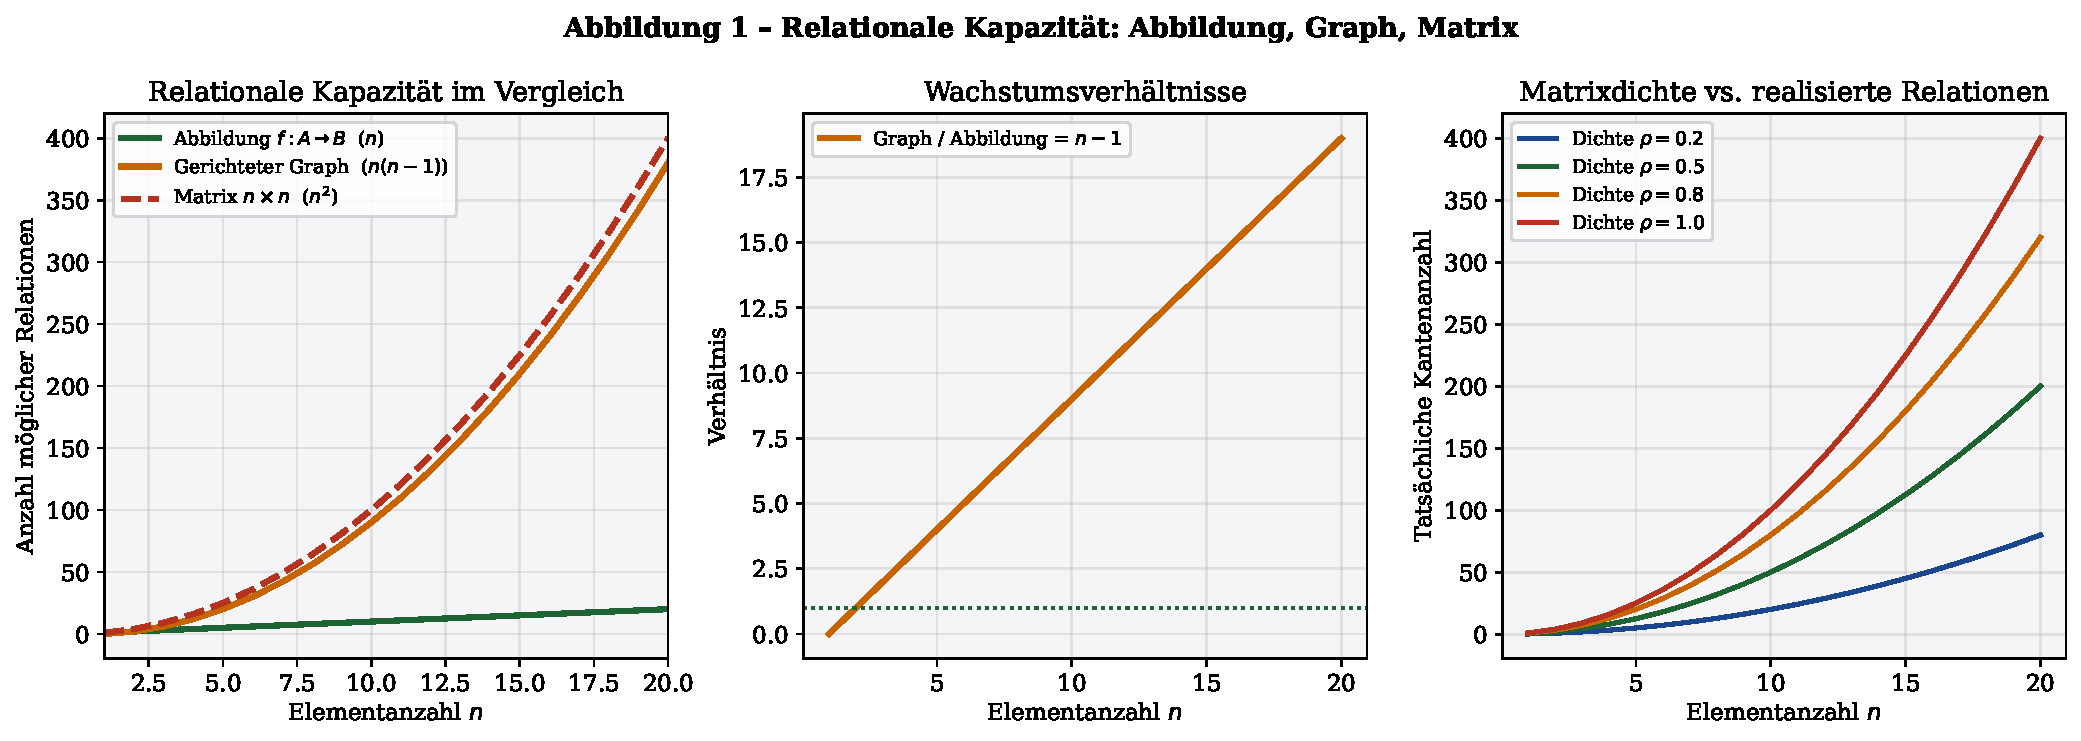
\includegraphics[width=0.97\textwidth]{figures/fig01_relational_capacity.pdf}
\caption{
  \textbf{Relationale Kapazität im Vergleich.}
  Das linke Teilbild zeigt das quadratische Wachstum der Matrixeinträge
  ($n^2$, rot gestrichelt), das lineare Wachstum einer Abbildung ($n$,
  grün) und das subquadratische Wachstum eines gerichteten Graphen ohne
  Schleifen ($n(n-1)$, orange) als Funktion der Elementanzahl $n$.
  Das mittlere Teilbild zeigt das Verhältnis Graph/Abbildung, das linear
  mit $n$ wächst. Das rechte Teilbild illustriert, wie verschiedene
  Matrixdichten $\rho \in \{0.2, 0.5, 0.8, 1.0\}$ die tatsächlich
  realisierten Relationen bestimmen. Für vollständig besetzte Matrizen
  ($\rho = 1$) wird die obere Schranke $n^2$ erreicht.
}
\label{fig:relcap}
\end{figure}

\begin{figure}[H]
\centering
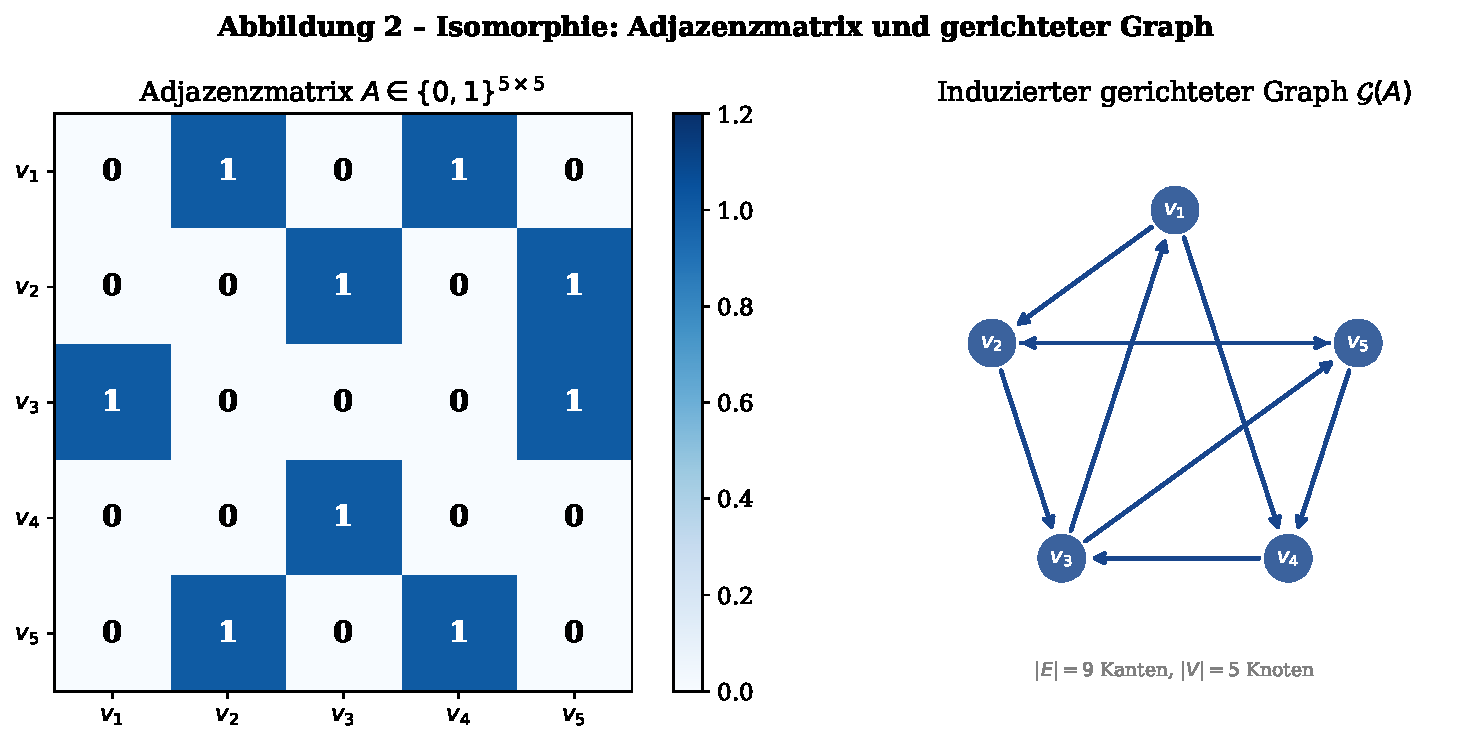
\includegraphics[width=0.97\textwidth]{figures/fig02_adjacency_graph.pdf}
\caption{
  \textbf{Adjazenzisomorphie: Matrix und Graph.}
  Links: Die $5 \times 5$-Adjazenzmatrix $A$ mit Einträgen 0 und 1.
  Rechts: Der zugehörige gerichtete Graph $\mathcal{G}(A)$ mit
  $|V| = 5$ Knoten und $|E|$ Kanten, arrangiert auf einem Kreis.
  Die Isomorphie $\Phi: A \mapsto \mathcal{G}(A)$ (Theorem~\ref{thm:iso})
  ist unmittelbar ablesbar: Jeder Nicht-Null-Eintrag $a_{ij} = 1$ entspricht
  genau einer Kante $v_i \to v_j$ im Graphen. Beide Darstellungen sind
  äquivalent und tragen dieselbe Information.
}
\label{fig:adjiso}
\end{figure}

\begin{figure}[H]
\centering
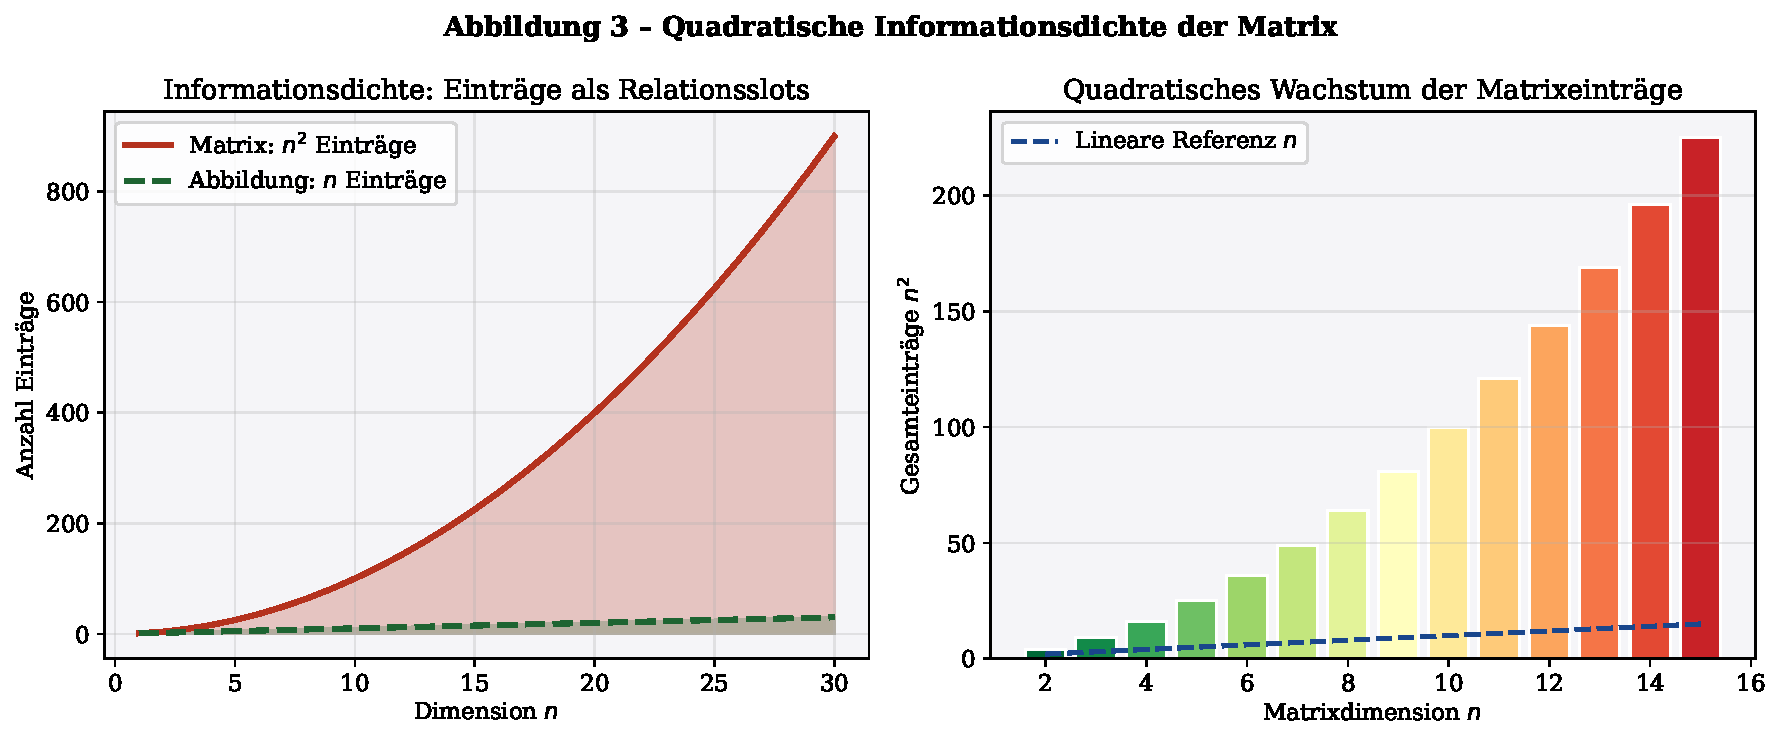
\includegraphics[width=0.97\textwidth]{figures/fig03_information_density.pdf}
\caption{
  \textbf{Quadratische Informationsdichte.}
  Links: Die quadratische Füllfläche $n^2$ (rot) übersteigt die lineare
  Referenz $n$ (grün, Abbildung) bereits bei $n = 5$ deutlich.
  Rechts: Balkendiagramm der tatsächlichen Einträge $n^2$ für
  Matrixdimensionen $n = 2, \ldots, 15$, farbkodiert nach Größe
  (Grün $\to$ Rot). Die blaue gestrichelte Linie zeigt die lineare
  Referenz. Das Diagramm verdeutlicht, dass selbst für moderate $n$
  die quadratische Dichte enorm ist: Bei $n = 15$ kodiert die Matrix
  225 Relationen, während eine Abbildung nur 15 trägt.
}
\label{fig:infodensity}
\end{figure}

\begin{figure}[H]
\centering
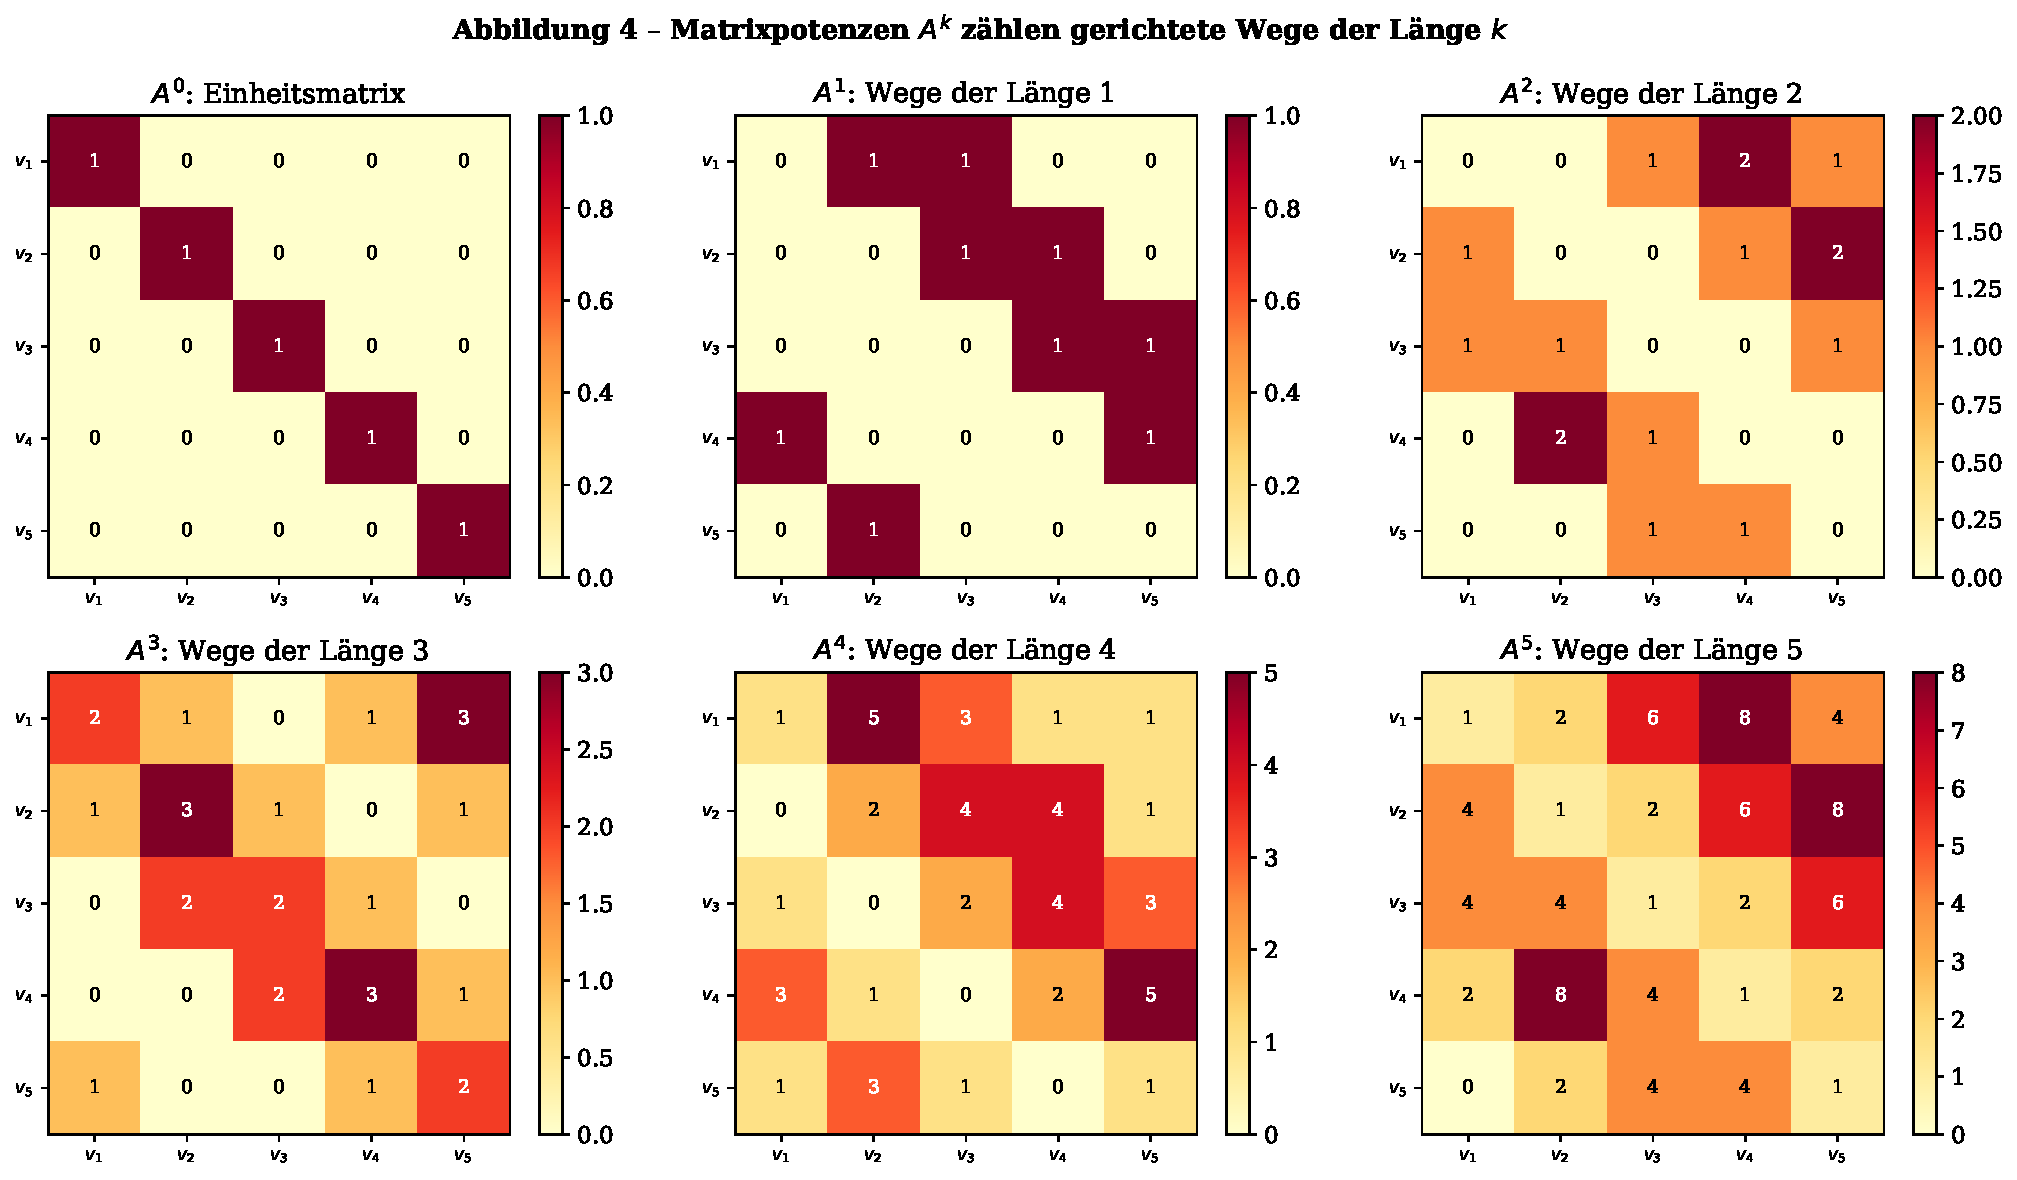
\includegraphics[width=0.97\textwidth]{figures/fig04_matrix_powers.pdf}
\caption{
  \textbf{Matrixpotenzen $A^k$ als Wegeanzahlen.}
  Sechs Heatmaps zeigen $A^0 = I$ bis $A^5$ für die
  $5 \times 5$-Beispielmatrix. Gemäß Theorem~\ref{thm:wege} kodiert
  $(A^k)_{ij}$ die Anzahl der gerichteten Wege der Länge $k$ von $v_i$
  nach $v_j$. $A^0 = I$ zeigt die triviale Einheitsrelation (nur Wege
  der Länge 0). Mit steigendem $k$ füllt sich die Matrix, bis für
  hinreichend großes $k$ alle erreichbaren Knotenpaare abgedeckt sind.
  Die Einträge wachsen für stark verbundene Graphen exponentiell.
}
\label{fig:matpow}
\end{figure}

\begin{figure}[H]
\centering
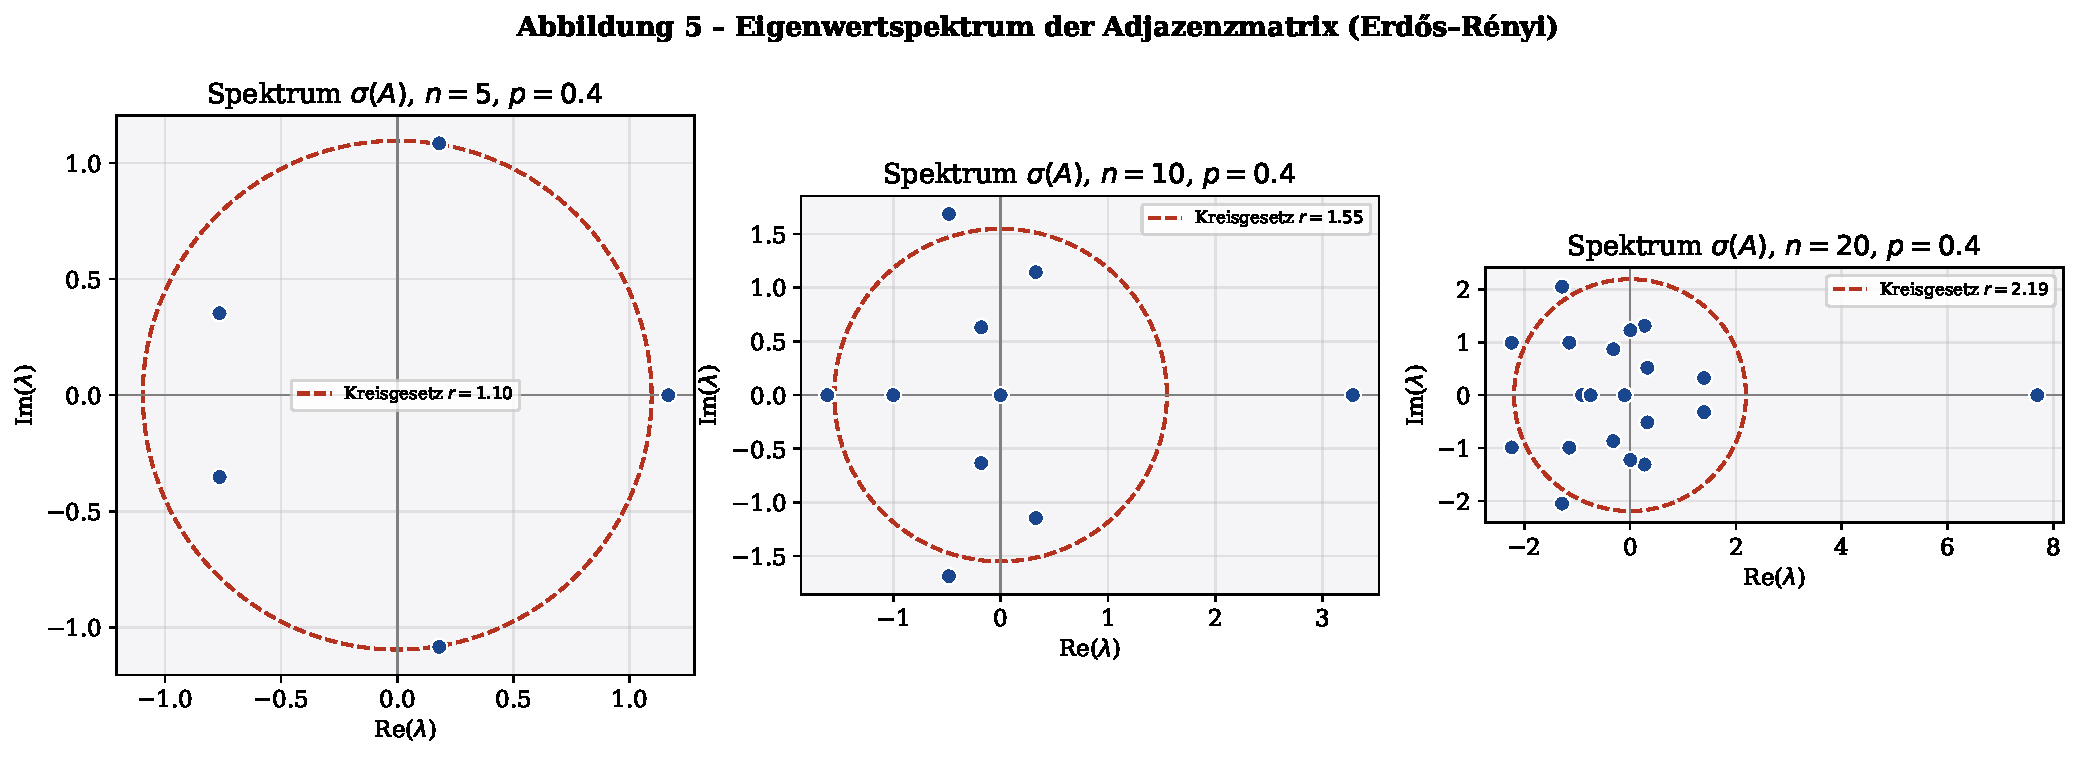
\includegraphics[width=0.97\textwidth]{figures/fig05_spectrum.pdf}
\caption{
  \textbf{Eigenwertspektrum von Erdős--Rényi-Adjazenzmatrizen.}
  Drei Plots zeigen das Spektrum $\sigma(A)$ in der komplexen Ebene für
  Zufallsadjazenzmatrizen mit $n \in \{5, 10, 20\}$ und Kantendichte
  $p = 0.4$. Die gestrichelten roten Kreise markieren den theoretischen
  Radius $r = \sqrt{n p(1-p)}$ des Kreisgesetzes (Wigner-Halbkreisgesetz
  für nichtsymmetrische Matrizen). Für wachsendes $n$ streut das Spektrum
  zunehmend und liegt konzentriert im Kreisbereich, was die
  Zufallsmatrixtheorie für sparse Graphen bestätigt.
}
\label{fig:spectrum}
\end{figure}

\begin{figure}[H]
\centering
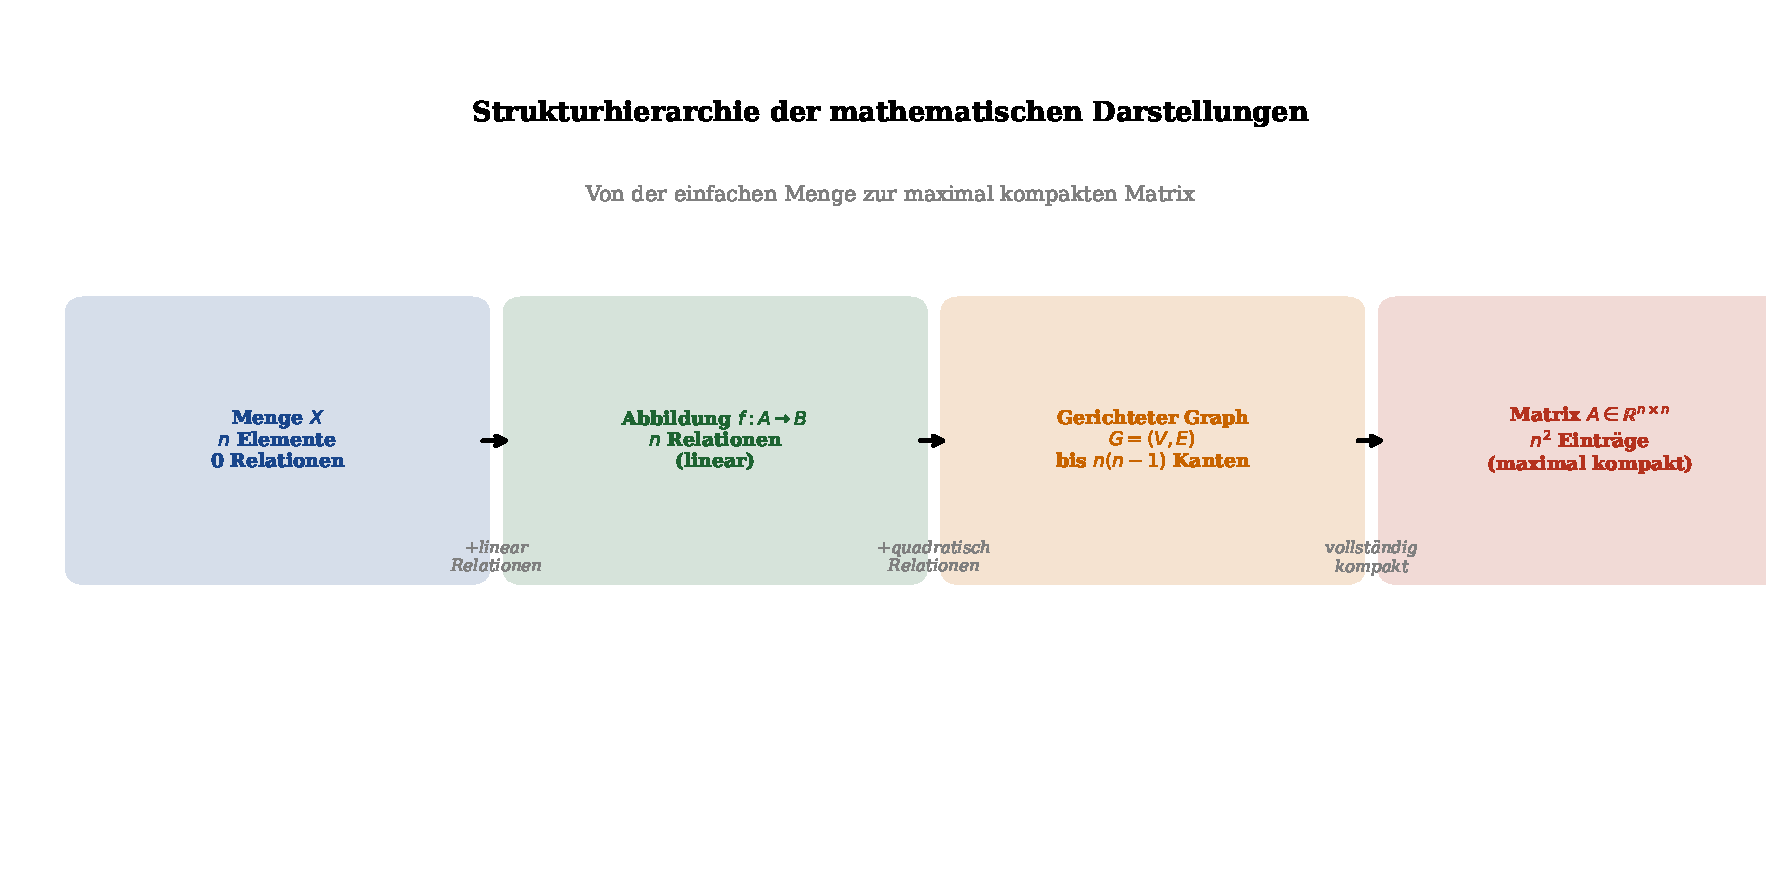
\includegraphics[width=0.95\textwidth]{figures/fig06_hierarchy.pdf}
\caption{
  \textbf{Strukturhierarchie der mathematischen Darstellungen.}
  Von links nach rechts: Menge (keine Relation), Abbildung (lineare
  Relationen), gerichteter Graph (quadratisch viele Kanten), Matrix
  (vollständig kompakt, $n^2$ Einträge). Pfeile zeigen die zunehmende
  relationale Mächtigkeit. Unterhalb der Pfeile stehen die
  Kapazitätssprünge. Die Matrix steht am rechten Ende der Hierarchie
  als maximal kompakte Struktur -- sie ist der Abschluss dieser Kette.
}
\label{fig:hierarchy}
\end{figure}

\begin{figure}[H]
\centering
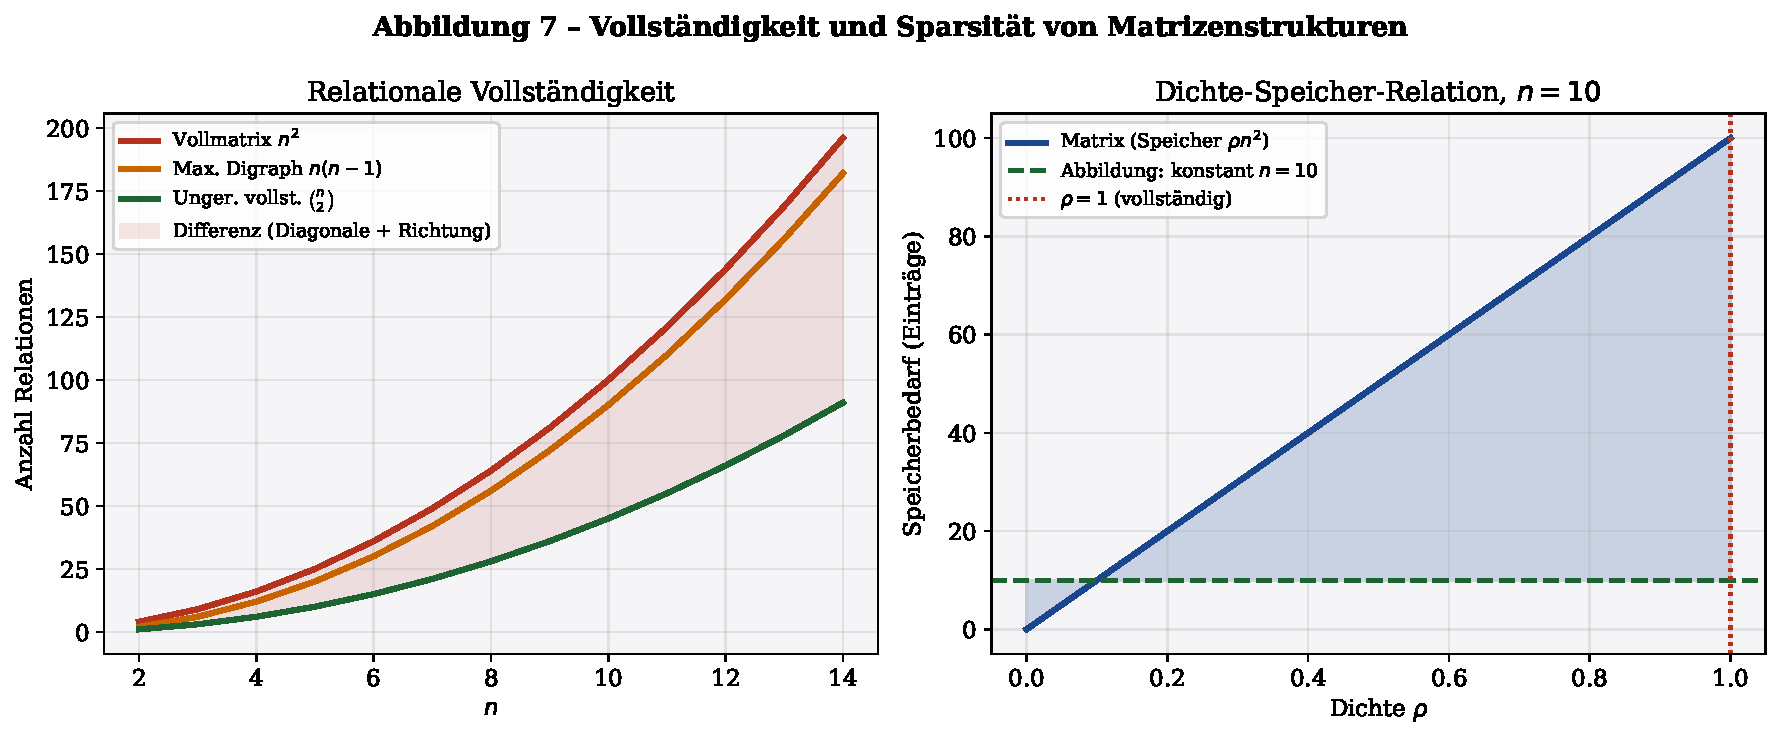
\includegraphics[width=0.97\textwidth]{figures/fig07_completeness.pdf}
\caption{
  \textbf{Vollständigkeit und Sparsität.}
  Links: Vergleich der Relationsanzahl für vollständige Matrix ($n^2$),
  maximalen Digraphen ($n(n-1)$) und vollständigen ungerichteten Graphen
  ($\binom{n}{2}$). Die rote Füllfläche illustriert den Beitrag von
  Diagonale und Richtungsinformation zur Ãœberlegenheit der Matrix.
  Rechts: Für $n = 10$ zeigt das Dichte-Speicher-Diagramm, wie der
  Speicherbedarf einer Matrix mit der Dichte $\rho$ skaliert. Die grüne
  gestrichelte Linie zeigt den konstanten Bedarf einer Abbildung.
  Erst bei sehr kleinen Dichten ($\rho \ll 1/n$) sind Sparse-Strukturen
  effizienter.
}
\label{fig:completeness}
\end{figure}

\begin{figure}[H]
\centering
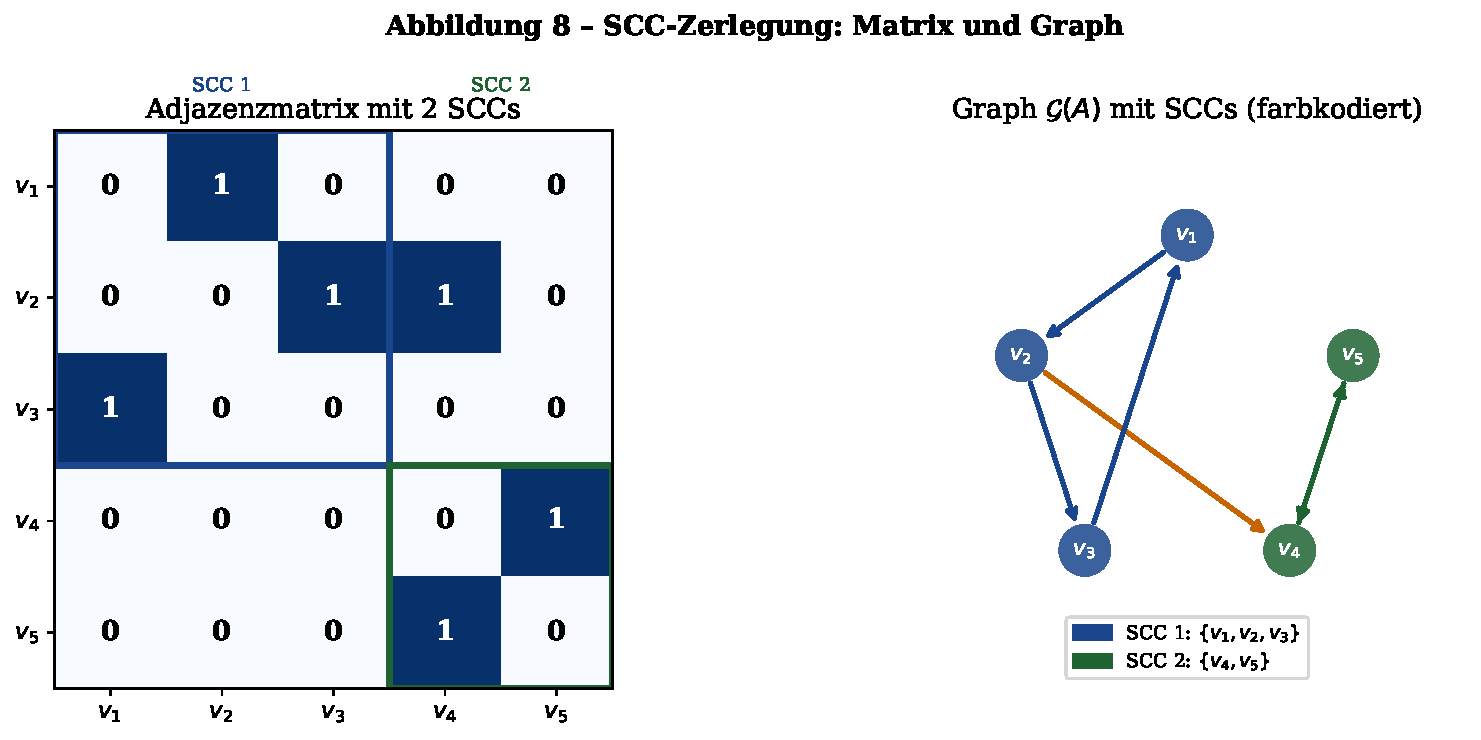
\includegraphics[width=0.97\textwidth]{figures/fig08_scc.pdf}
\caption{
  \textbf{SCC-Zerlegung von Matrix und Graph.}
  Links: Die $5 \times 5$-Adjazenzmatrix mit zwei hervorgehobenen
  Diagonalblöcken (blau: SCC~1 = $\{v_1,v_2,v_3\}$,
  grün: SCC~2 = $\{v_4,v_5\}$) entsprechend Theorem~\ref{thm:scc_block}.
  Rechts: Der zugehörige Graph mit farbkodierten Knoten. Die
  Blockdreiecksstruktur der permutierten Matrix ist direkt sichtbar.
  Die Inter-SCC-Kante (orange) verläuft nur in topologischer Richtung
  (von SCC~1 nach SCC~2), nie zurück.
}
\label{fig:scc}
\end{figure}

\begin{figure}[H]
\centering
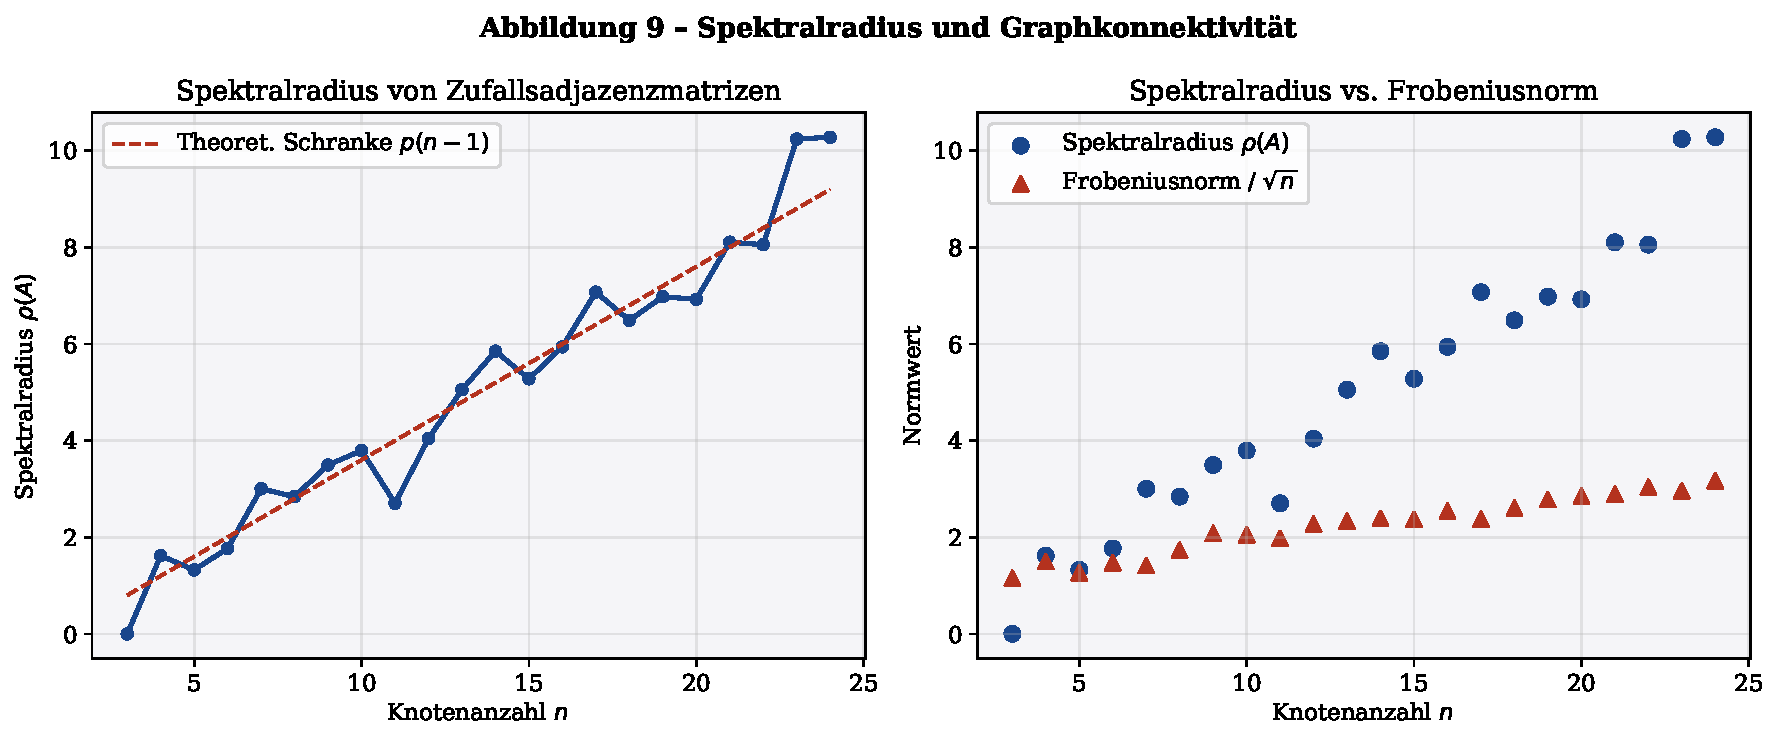
\includegraphics[width=0.97\textwidth]{figures/fig09_spectral_radius.pdf}
\caption{
  \textbf{Spektralradius und Graphkonnektivität.}
  Links: Spektralradius $\rho(A)$ als Funktion der Knotenanzahl $n$
  (blau) im Vergleich zur theoretischen Schranke $p(n-1)$ (rot gestrichelt).
  Der Spektralradius wächst sublinear in $n$ für feste Dichte $p$.
  Rechts: Vergleich von Spektralradius und normierter Frobeniusnorm
  $\|A\|_F / \sqrt{n}$ -- beide Größen zeigen ähnliches Wachstum, was
  die Konsistenz der Matrixnormen illustriert.
}
\label{fig:specrad}
\end{figure}

\begin{figure}[H]
\centering
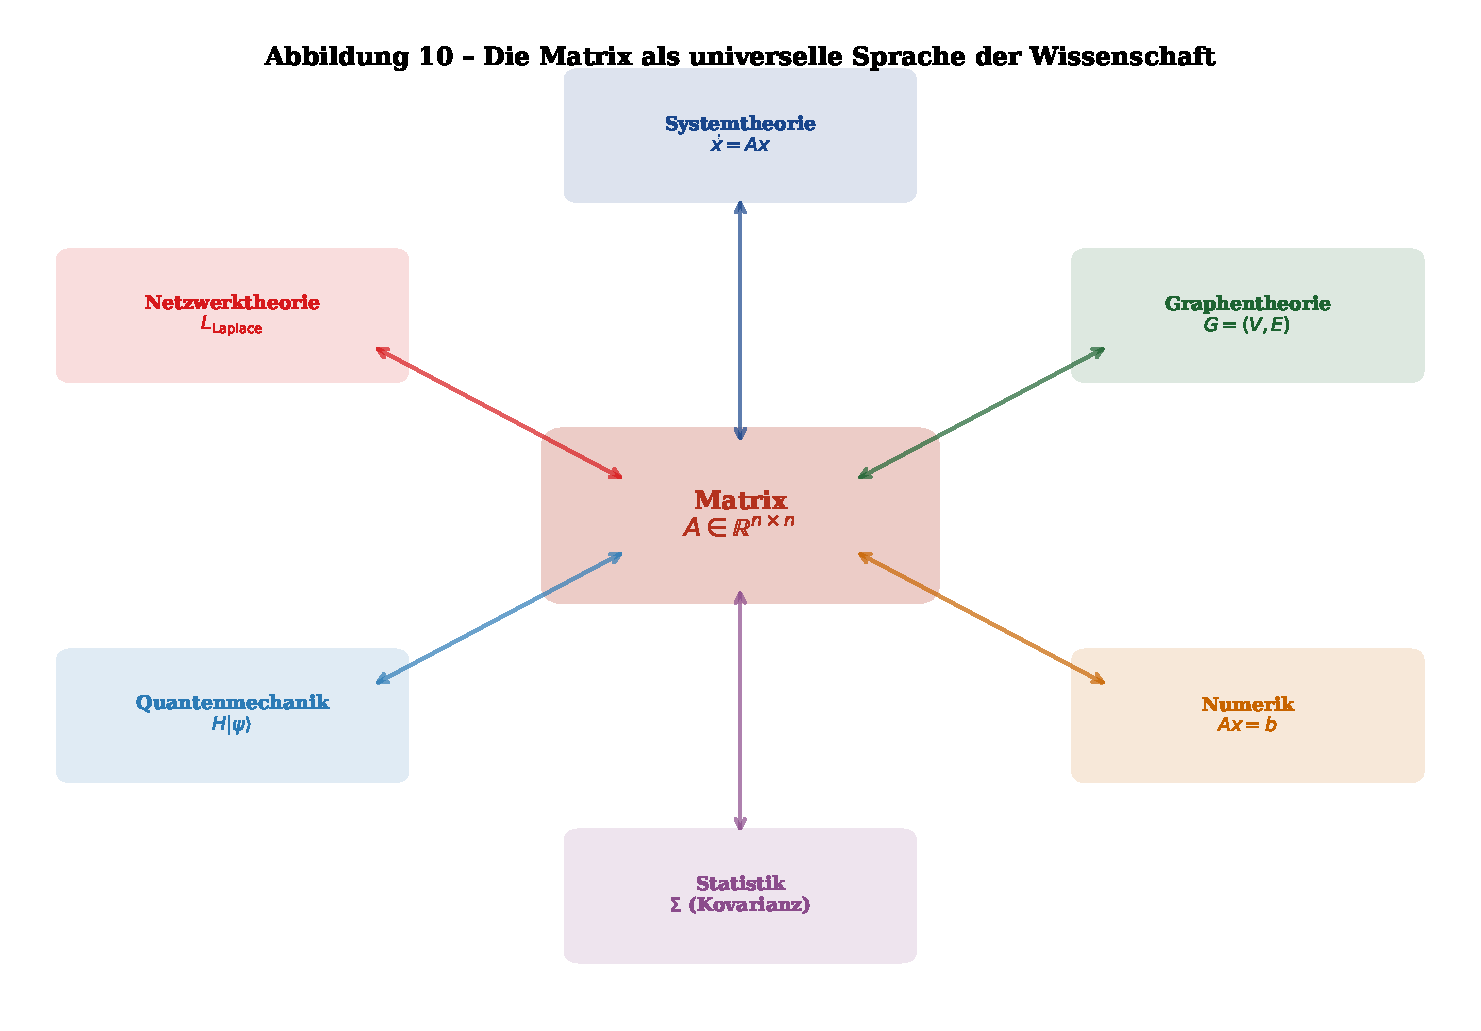
\includegraphics[width=0.85\textwidth]{figures/fig10_universal.pdf}
\caption{
  \textbf{Die Matrix als universelle Sprache der Wissenschaft.}
  Die zentrale Matrix $A \in \R^{n \times n}$ (rot) steht im Mittelpunkt
  von sechs Wissenschaftsdisziplinen: Systemtheorie, Graphentheorie,
  Numerik, Statistik (Kovarianzmatrix), Quantenmechanik (Hamiltonoperator)
  und Netzwerktheorie (Laplace-Matrix). Die bidirektionalen Pfeile
  symbolisieren, dass jede Disziplin die Matrix nutzt und ihr eigene
  Interpretationen verleiht. Diese universelle Darstellungskraft ist eine
  direkte Konsequenz der maximalen relationalen Kapazität aus
  Theorem~\ref{thm:maxkompakt}.
}
\label{fig:universal}
\end{figure}

% ============================================================
\section{Ausblick}
\label{sec:ausblick}
% ============================================================

Die vorliegende Arbeit hat die fundamentale Stellung der quadratischen
Matrix als maximal kompakte mathematische Darstellung nachgewiesen. Die
Ergebnisse -- Theorem~\ref{thm:maxkompakt} (maximale relationale
Kapazität), Theorem~\ref{thm:iso} (Adjazenzisomorphie) und
Theorem~\ref{thm:wege} (Wegeanzahlsatz) -- bilden ein kohärentes
Fundament, das zahlreiche weiterführende Forschungsrichtungen eröffnet.
Dieser Ausblick entwickelt diese Perspektiven in sechs großen
Themenblöcken.

\subsection{Verallgemeinerungen des Kompaktheitsbegriffs}
\label{subsec:verallg}

\subsubsection*{Tensoren als Kompaktheitsverallgemeinerung}

Die natürliche Verallgemeinerung der Matrix ist der Tensor
$\mathcal{T} \in \R^{n_1 \times n_2 \times \cdots \times n_k}$. Für
einen $k$-Tensor über einer $n$-elementigen Grundmenge gilt
$\kappa(\mathcal{T}) = n^k$. Die Kompaktheitshierarchie
\[
  n \;\ll\; n^2 \;\ll\; n^3 \;\ll\; \cdots \;\ll\; n^k
\]
zeigt, dass Tensoren höherer Ordnung noch mächtigere Relationen
kodieren können. Die Frage lautet: Welche algebraischen Strukturen
und Algorithmen sind auf Tensoren übertragbar, und wie verhält sich
die Adjazenzisomorphie (Theorem~\ref{thm:iso}) in höheren Dimensionen?
Hypergraphen $\mathcal{H} = (V, \mathcal{E})$, bei denen Hyperkanten
mehr als zwei Knoten verbinden, sind die graphentheoretischen Analoga
von Tensoren höherer Ordnung. Ein vollständiges Analogon von
Theorem~\ref{thm:iso} für Hypergraphen und Tensoren steht noch aus.

\subsubsection*{Unendlichdimensionale Verallgemeinerung}

Die vorliegende Arbeit beschränkte sich auf $\vA \in \R^{n \times n}$
mit $n < \infty$. Die unendlichdimensionale Verallgemeinerung führt
auf beschränkte lineare Operatoren $T: \mathcal{H} \to \mathcal{H}$ auf
Hilberträumen $\mathcal{H}$. Die Spektraltheorie dieser Operatoren
(Spektralmaß, spektrale Zerlegung \citep{riesz1955}) ist erheblich
reichhaltiger: Neben dem Punktspektrum gibt es kontinuierliches und
Residualspektrum. Eine präzise Definition der ``relationalen Kapazität''
für Operatoren und ein Analogon zu Theorem~\ref{thm:maxkompakt} in
unendlicher Dimension wäre ein wichtiger Schritt.

\subsubsection*{Matrizenstrukturen mit Zusatzeigenschaften}

Innerhalb des Raumes $\mathcal{M}_n(\R)$ definieren strukturelle
Einschränkungen interessante Unterräume: symmetrische Matrizen
($\dim = n(n+1)/2$), schiefsymmetrische Matrizen ($\dim = n(n-1)/2$),
Toeplitz-Matrizen, zirkulante Matrizen, Hankel-Matrizen, etc.
Jede dieser Unterklassen hat charakteristische spektrale Eigenschaften
und effiziente Algorithmen. Eine systematische Theorie, welche
Kompaktheits- und Darstellungseigenschaften bei diesen Einschränkungen
erhalten bleiben, fehlt noch vollständig.

\subsection{Erweiterungen der Adjazenzisomorphie}
\label{subsec:adj_ausblick}

\subsubsection*{Gewichtete und gemischte Graphen}

Theorem~\ref{thm:iso} stellt die volle Bijektivität für gewichtete
Digraphen fest. Viele praktisch relevante Graphklassen -- gemischte
Graphen (mit gerichteten und ungerichteten Kanten), probabilistische
Graphen (Bayessche Netze), zeitvariante Graphen -- besitzen keine
triviale Matrizenentsprechung. Die Frage, welche Matrizenklasse die
``natürliche'' Darstellung für jeden dieser Graphtypen ist, ist
weitgehend offen und hat direkte Implikationen für algorithmische
Effizienz.

\subsubsection*{Graphisomorphieproblem und Matrizenperspektive}

Das Graphisomorphieproblem (GIP) -- gegeben zwei Graphen $G_1, G_2$,
existiert eine Knotenbijektion, die $G_1$ in $G_2$ überführt? -- ist
eines der bekanntesten offenen Probleme der Komplextheorie (bekannt: in
$\mathrm{NP}$, Babai \citep{babai2016} hat einen quasipolynomiellen
Algorithmus $n^{O(\log n)}$ gezeigt). In Matrizensprache: Existiert
eine Permutationsmatrix $\vP$ mit $\vP \vA_1 \vP^\T = \vA_2$?
Die Kompaktheitstheorie der Matrix könnte neue invariantenbasierte
Ansätze liefern: spektrale Invarianten ($\spec(\vA)$), Knotengrade
($\bm{d}$), Spur von Potenzen ($\tr(\vA^k)$) sind polynomiell
berechenbare Kandidaten für vollständige Isomorphieinvarianten --
der Nachweis ihrer Vollständigkeit ist jedoch offen.

\subsubsection*{Subgraph Algorithmus und strukturelle Äquivalenz}

Der Subgraph Algorithmus \citep{epp2026subgraph} nutzt signaturbasierte
Matrizenkodierung zur Graphisomorphieerkennung mit Laufzeit
$\Theta(n^3)$. Eine wichtige offene Frage ist die Charakterisierung
der Klasse von Graphen, für die der Algorithmus korrekte
Negativzertifikate liefert. In Verbindung mit der Adjazenzisomorphie
(Theorem~\ref{thm:iso}) stellt sich die Frage: Welche Matrizenklassen
haben \emph{vollständige} Signaturinvarianten unter der Subgraph-Kodierung?
Dies würde die Grenze zwischen polynomiell lösbaren und schwierigen
Instanzen des GIP schärfer ziehen.

\subsection{Dynamische und zeitvariante Matrizensysteme}
\label{subsec:dynamisch}

\subsubsection*{Zeitvariante Systemmatrizen}

Die Zustandsraumdarstellung~\eqref{eq:zustandsraum} mit konstanter Matrix
$\vA$ ist der einfachste Fall. Reale Systeme sind häufig zeitvariant:
$\dot{\vx} = \vA(t)\vx$. Die Lösung via Peano-Baker-Reihe
\[
  \vx(t) = \Phi(t, t_0)\vx_0, \qquad
  \Phi(t,t_0) = \vI + \int_{t_0}^t \vA(\tau_1)\,d\tau_1
    + \int_{t_0}^t \vA(\tau_1)\int_{t_0}^{\tau_1}\vA(\tau_2)\,d\tau_2\,d\tau_1 + \cdots
\]
ist direkt mit den Matrixpotenzen aus Theorem~\ref{thm:wege} verwandt.
Eine graphentheoretische Interpretation der Transitionsmatrix
$\Phi(t,t_0)$ -- als zeitabhängiger Graph mit zeitlich variierenden
Kantengewichten -- ist konzeptionell klar, aber algorithmisch noch
nicht vollständig erschlossen.

\subsubsection*{Nichtlineare Systeme und Koopman-Operator}

Für nichtlineare Systeme $\dot{\vx} = f(\vx)$ bietet der
\emph{Koopman-Operator} $\mathcal{K}$ eine lineare, aber
unendlichdimensionale Darstellung: $\mathcal{K} \phi = \phi \circ f_t$
für Observablen $\phi: \R^n \to \R$. Datengetriebene Methoden
(EDMD -- Extended Dynamic Mode Decomposition) approximieren $\mathcal{K}$
durch endliche Matrizen $\hat{\vK} \in \R^{m \times m}$ ($m \gg n$).
Die Frage lautet: Wie viel relationale Information geht bei der
Projektion $\mathcal{K} \to \hat{\vK}$ verloren, und wie hängt dies mit
der Kompaktheitstheorie aus Theorem~\ref{thm:maxkompakt} zusammen?

\subsubsection*{Matrizensequenzen und Markov-Ketten}

Eine \emph{stochastische Matrix} $\vP \in [0,1]^{n \times n}$ mit
$\sum_j p_{ij} = 1$ beschreibt einen Markov-Prozess. Die $k$-Schritt-
Ãœbergangswahrscheinlichkeiten sind $(P^k)_{ij}$, analog zu
Theorem~\ref{thm:wege}. Langfristiges Verhalten (stationäre Verteilung)
ist durch den dominanten Eigenvektor (Perron-Frobenius,
Theorem~\ref{thm:pf}) bestimmt. Die kompakte Matrizendarstellung erlaubt
hier nicht nur analytische Aussagen, sondern auch effiziente numerische
Simulation großer Markov-Ketten.

\subsection{Informatik, Komplexitätstheorie und Algorithmik}
\label{subsec:algo_ausblick}

\subsubsection*{Matrizenmultiplikation und Coppersmith-Winograd}

Die Matrizenmultiplikation $\vA \cdot \vB$ ist das zentrale algorithmische
Primitiv. Der triviale Algorithmus benötigt $O(n^3)$ Operationen. Der
beste bekannte Algorithmus (Williams, 2024) erreicht $O(n^{2.371552})$.
Die fundamentale Frage $\omega = 2$? (ob Matrizenmultiplikation in fast
quadratischer Zeit möglich ist) ist offen. In Verbindung mit der
Kompaktheitstheorie: Da die Matrix $n^2$ Einträge trägt, bildet
$O(n^2)$ die \emph{informationstheoretische Untergrenze} für jeden
nicht-trivialen Matrizenalgorithmus (er muss jeden Eintrag mindestens
einmal lesen). Die Lücke zwischen $n^2$ und $n^\omega$ misst den
algorithmischen ``Overhead'' relativ zur relationalen Kompaktheit.

\subsubsection*{Spärliche Matrizen und Kompressionsschemata}

Für sparse Matrizen ($\rho \ll 1$) ist die volle $n \times n$-Darstellung
suboptimal. Kompressionsschemata (CSR -- Compressed Sparse Row, CSC, COO)
reduzieren den Speicherbedarf auf $O(m)$ für $m \ll n^2$ Nicht-Null-Einträge.
Die vorliegende Kompaktheitstheorie gilt für \emph{dichte} Matrizen; eine
erweiterte Theorie sollte quantifizieren, bei welcher Dichte $\rho^*(n)$
der Ãœbergang von dichter zu sparser Darstellung optimal ist, und wie
dies die relationale Kapazität beeinflusst.

\subsubsection*{Quantencomputing und Matrizenoperationen}

Quantenalgorithmen (HHL-Algorithmus für lineare Gleichungssysteme,
Quantensingulärwertzerlegung) versprechen exponentielle Beschleunigungen
für bestimmte Matrizenprobleme. Die Kompaktheitstheorie muss in diesem
Kontext neu bewertet werden: Ein $n$-Qubit-Zustand kodiert $2^n$
Amplituden, ein analoges ``Quantenmatrizenregister'' könnte $4^n$
Einträge tragen. Das Verhältnis von klassischer Matrizenkompaktheit
($n^2$) zu Quantenrepräsentation ($4^n$) ist eine offene Frage von
fundamentaler Bedeutung.

\subsection{Netzwerkwissenschaft und komplexe Systeme}
\label{subsec:netzwerk}

\subsubsection*{Multilayer-Netzwerke}

Reale komplexe Netzwerke (soziale Netzwerke, biologische Netze,
Infrastrukturnetzwerke) sind \emph{Multilayer-Netzwerke}: Dieselben
Knoten sind durch mehrere Relationstypen verbunden. Die mathematische
Darstellung ist ein Tensor $\mathcal{A} \in \R^{n \times n \times L}$
($L$ Layer) oder äquivalent eine $nL \times nL$-Superadjazenzmatrix.
Die Kompaktheitstheorie für diese Strukturen -- Wie viele Relationen
kann ein Multilayer-Netzwerk tragen? Welche Algorithmen sind übertragbar?
-- ist ein aktives Forschungsgebiet.

\subsubsection*{Graphneuronale Netze und Lernbare Adjazenzmatrizen}

Graphneuronale Netze (GNNs) lernen direkt auf Graphen, indem sie
Knotenrepräsentationen durch iterative Nachrichtenübermittlung
aggregieren. Die Adjazenzmatrix ist die fundamentale Struktur der
Nachrichtenübermittlung: $H^{(k+1)} = \sigma(\tilde{\vA} H^{(k)} W^{(k)})$,
wobei $\tilde{\vA}$ die normierte Adjazenzmatrix, $H^{(k)}$ die
Knotenmerkmale und $W^{(k)}$ lernbare Gewichte sind. Die Kompaktheit
der Matrix bestimmt direkt die Ausdruckskraft des GNN: Ein GNN, das nur
auf der Adjazenzmatrix operiert, kann maximal so viele strukturelle
Muster unterscheiden, wie die Matrix kodiert. Die Verbindung zwischen
Theorem~\ref{thm:maxkompakt} und der Ausdruckskraftanalyse von GNNs
(Weisfeiler-Leman-Hierarchie) ist eine wichtige offene Frage.

\subsubsection*{Zufallsmatrizentheorie und Schwellenphänomene}

Für Erdős--Rényi-Zufallsgraphen $G(n,p)$ zeigt die Spektraltheorie
charakteristische Schwellenphänomene: Bei $p = \log(n)/n$ wird der
Graph fast sicher zusammenhängend; bei $p = 1/n$ entsteht der größte
Zusammenhangsgraph. Diese Schwellen spiegeln sich im Spektrum von
$\vA_G$ wider ($\lambda_2(\vL) > 0$ iff. Zusammenhang). Eine
vollständige spektrale Charakterisierung aller Schwellenphänomene
als Matrixeigenschaften wäre ein wichtiger Fortschritt in der
Zufallsmatrizentheorie.

\subsection{Biologie, Physik und Interdisziplinäre Anwendungen}
\label{subsec:interdisziplin}

\subsubsection*{Biologische Netzwerke und Genregulation}

Genregulationsnetzwerke werden durch Adjazenzmatrizen beschrieben:
$(A_{\rm GRN})_{ij} = $ Akti\-vierungs-/Repressionsstärke von Gen $j$ auf
Gen $i$. Die Kompaktheit der Matrix erlaubt es, alle paarweisen
regulatorischen Interaktionen in einem $n \times n$-Array zu kodieren.
Die SCC-Zerlegung (Theorem~\ref{thm:scc_block}) identifiziert regulatorische
Module (Feedback-Schleifen, Master-Regulatoren). Der Perron-Frobenius-Eigenwert
(Theorem~\ref{thm:pf}) korrespondiert mit der dominanten
Proliferationsrate. Anwendungen in der Systembiologie -- insbesondere
beim Verständnis von Krebsgenomik, Stammzell-Reprogrammierung und
Antibiotikaresistenz -- sind direkt angeschlossen.

\subsubsection*{Neuronale Konnektivitätsmatrizen}

In den Neurowissenschaften kodiert die Konnektivitätsmatrix (Strukturkonnektom
oder funktionales Konnektom) die synaptischen Verbindungen bzw.
Korrelationen zwischen Hirnregionen. Für den Menschen umfasst das
strukturelle Konnektom ca. $n \approx 10^{11}$ Neuronen -- eine Matrix
mit $n^2 \approx 10^{22}$ Einträgen, die natürlich sparse ist.
Dennoch ist die theoretische Maximalkapazität $n^2$ der entscheidende
Referenzpunkt für Effizienzanalysen. Spektraleigenschaften des
Konnektoms (Synchronisation, kritische Dynamik, Eigenvektor-Konnektivität)
sind aktive Forschungsgegenstände.

\subsubsection*{Physikalische Systeme und Transfermatrizen}

In der statistischen Physik beschreibt die \emph{Transfermatrix}
$\vT$ eines eindimensionalen Gittermodells (Ising-Modell, Potts-Modell)
die Wechselwirkungen benachbarter Gitterpunkte. Die Zustandssumme des
Systems ist $Z = \tr(\vT^N)$ für $N$ Gitterpunkte -- ein direktes
Analogon zu Theorem~\ref{thm:spur}. Der größte Eigenwert von $\vT$
(Perron-Frobenius) bestimmt die freie Energie; die Spektrallücke
kodiert die Korrelationslänge. Die Verbindung zwischen
Kompaktheitstheorie und statistischer Physik ist damit tief und
mathematisch präzise.

\subsection{Philosophische und erkenntnistheoretische Dimensionen}
\label{subsec:philosophie}

\subsubsection*{Die Matrix als epistemische Struktur}

Die Tatsache, dass nahezu alle Bereiche der modernen Mathematik und
Naturwissenschaften auf die Matrix als Grunddarstellung zurückgreifen,
ist keine bloße Konvention. Sie folgt aus dem Kompaktheitssatz
(Theorem~\ref{thm:maxkompakt}): Die Matrix ist die \emph{effizienteste}
Weise, alle möglichen Beziehungen zwischen $n$ Entitäten zu kodieren.
In der Erkenntnistheorie entspricht dies der Aussage, dass die Matrix
die minimale kognitive Einheit ist, die vollständige relationale
Information trägt. Das Konzept der \emph{epistemischen Wolke}
\citep{epp2026sysstate} -- die Gesamtheit aller möglichen Zustände
und ihrer Übergänge -- findet in der Adjazenzmatrix seine natürliche
mathematische Verkörperung.

\subsubsection*{Graphentheoretisches Denken als kognitive Grundlage}

Graphentheoretisches Denken ist eine natürliche kognitive Strategie:
Entitäten werden als Knoten, Beziehungen als Kanten repräsentiert.
Die Adjazenzisomorphie (Theorem~\ref{thm:iso}) zeigt, dass dieses
kognitive Framework \emph{exakt äquivalent} zur algebraischen
Matrizendarstellung ist. Keine Information geht verloren; beide
Darstellungen sind vollständig austauschbar. Dies bedeutet, dass
graphentheoretisches Denken nicht nur eine didaktische Hilfe ist,
sondern eine mathematisch vollständige Alternative zur
Matrizenalgebra -- mit dem Vorteil der visuellen Intuition und dem
Nachteil der eingeschränkten algebraischen Zugänglichkeit.

\subsubsection*{Einheit der Mathematik durch die Matrix}

Die universelle Darstellungskraft der Matrix (Abschnitt~\ref{sec:anwendungen},
Abbildung~\ref{fig:universal}) suggeriert, dass die Matrix ein
\emph{unifier} der Mathematik ist: ein gemeinsames Substrat, auf dem
Algebra, Analysis, Geometrie, Topologie und Kombinatorik gemeinsam
operieren. Dies ist nicht zufällig, sondern folgt aus dem Kompaktheitssatz:
Weil die Matrix die reichste elementare Struktur ist, können in ihr
die Grundstrukturen aller Teilgebiete kodiert werden. Eine vollständige
``Theorie der Mathematik als Matrizentheorie'' -- analog zu Hilberts
Programm für die Arithmetik -- wäre ein spekulatives, aber
intellektuell reizvolles Forschungsprogramm.

\subsection{Offene Probleme und Forschungsagenda}
\label{subsec:agenda}

Die folgende Tabelle fasst die wichtigsten offenen Probleme und
Forschungsrichtungen zusammen:

\begin{table}[H]
\centering
\caption{Forschungsagenda: Kurzfristige, mittelfristige und langfristige Ziele}
\label{tab:agenda}
\begin{tabular}{>{\raggedright\arraybackslash}p{2.5cm}
                >{\raggedright\arraybackslash}p{5.0cm}
                >{\raggedright\arraybackslash}p{5.5cm}}
\toprule
\textbf{Horizont} & \textbf{Thema} & \textbf{Forschungsziel} \\
\midrule
Kurzfristig & Tensorkompaktheit & Analogon Theorem~\ref{thm:maxkompakt} für $k$-Tensoren \\
 & Operator-Kapazität & Kapazitätsdefinition für $T: \mathcal{H} \to \mathcal{H}$ \\
 & Signatur-Vollständigkeit & Vollständigkeit der Subgraph-Signatur \citep{epp2026subgraph} \\
 & Sparse-Schwelle & Optimale Dichteschwelle $\rho^*(n)$ \\
\midrule
Mittelfristig & GNN-Ausdruckskraft & Verbindung Kompaktheit -- WL-Hierarchie \\
 & Zeitvariante Adj. & Graphdarstellung von Peano-Baker-Reihe \\
 & Koopman-Kompaktheit & Verlust bei $\mathcal{K} \to \hat{\vK}$ \\
 & Multilayer-Theorie & Kompaktheit von $\mathcal{A} \in \R^{n \times n \times L}$ \\
\midrule
Langfristig & Quantenmatrizentheorie & Kompaktheit von Quantenregistern \\
 & $\omega = 2$? & Matrizenmultiplikationsoptimalität \\
 & Einheitsprogramm & Mathematik als Matrizentheorie \\
 & Topologische Invarianten & Persistente Homologie vs. Spektrum \\
\bottomrule
\end{tabular}
\end{table}

\subsection{Schlussbetrachtung}
\label{subsec:schluss}

Die quadratische Matrix ist nicht nur ein praktisches Rechenhilfsmittel,
sondern die \emph{kanonische} und \emph{maximal effiziente} Darstellung
von Relationen in der Mathematik. Theorem~\ref{thm:maxkompakt} zeigt,
dass ihre $n^2$ Einträge die theoretische Obergrenze der relationalen
Kapazität für eine $n$-elementige Grundmenge realisieren. Theorem~\ref{thm:iso}
zeigt, dass die Verbindung zur Graphentheorie keine Analogie ist, sondern
eine exakte mathematische Isomorphie -- Matrizen und gewichtete Digraphen
sind dieselbe mathematische Struktur in zwei Darstellungskleidern.

Die Konsequenzen sind weitreichend: Alle graphentheoretischen Algorithmen
sind Matrizenalgorithmen und umgekehrt. Alle Matrizeneigenschaften haben
graphentheoretische Interpretationen. Die Spektraltheorie verbindet
algebraische Invarianten (Eigenwerte) mit kombinatorischen Eigenschaften
(Wegeanzahlen, Konnektivität, Zyklenstruktur). Und die universelle
Darstellungskraft der Matrix erklärt, warum sie in so vielen Disziplinen
die zentrale Rolle spielt.

Zukünftige Arbeiten werden diese Fundamente in höhere Dimensionen
(Tensoren), unendliche Räume (Operatoren), zeitliche Dynamik und
interdisziplinäre Anwendungen ausweiten. Das Ziel ist eine vollständige
\emph{Kompaktheitstheorie mathematischer Darstellungen} -- eine Theorie,
die quantifiziert, wie viel Information welche Struktur tragen kann, und
welche algorithmischen, kognitiven und epistemischen Konsequenzen dies
hat. Die vorliegende Arbeit ist der erste Schritt auf diesem Weg.

% ============================================================
\bibliographystyle{plainnat}
\begin{thebibliography}{99}
	
	\bibitem[Epp(2026a)]{epp2026subgraph}
	Epp, S. (2026).
	\newblock \textit{Der Subgraph Algorithmus}. Verfügbar unter
	\url{https://github.com/hjstephan86/science}.
	
	\bibitem[Epp(2026b)]{epp2026sysstate}
	Epp, S. (2026).
	\newblock \textit{Zustandsklassen dynamischer Systeme und ihre wirtschaftlichen
		Implikationen}. April 2026
	
	\bibitem[Babai(2016)]{babai2016}
	Babai, L. (2016).
	\newblock Graph isomorphism in quasipolynomial time.
	\newblock In \textit{Proceedings of the 48th Annual ACM STOC}, pages 684--697.
	
	\bibitem[Barabási(2016)]{barabasi2016}
	Barabási, A.-L. (2016).
	\newblock \textit{Network Science}.
	\newblock Cambridge University Press.
	
	\bibitem[Bollobás(1998)]{bollobas1998}
	Bollobás, B. (1998).
	\newblock \textit{Modern Graph Theory}.
	\newblock Springer.
	
	\bibitem[Brogan(1991)]{brogan1991}
	Brogan, W.~L. (1991).
	\newblock \textit{Modern Control Theory}, 3rd ed.
	\newblock Prentice Hall, Englewood Cliffs, NJ.
	
	\bibitem[Chung(1997)]{chung1997}
	Chung, F.~R.~K. (1997).
	\newblock \textit{Spectral Graph Theory}.
	\newblock American Mathematical Society.
	
	\bibitem[Cormen et~al.(2009)]{cormen2009}
	Cormen, T.~H., Leiserson, C.~E., Rivest, R.~L., and Stein, C. (2009).
	\newblock \textit{Introduction to Algorithms}, 3rd ed.
	\newblock MIT Press.
	
	\bibitem[Diestel(2017)]{diestel2017}
	Diestel, R. (2017).
	\newblock \textit{Graph Theory}, 5th ed.
	\newblock Springer.
	
	\bibitem[Estrada(2012)]{estrada2012}
	Estrada, E. (2012).
	\newblock \textit{The Structure of Complex Networks}.
	\newblock Oxford University Press.
	
	\bibitem[Godsil and Royle(2001)]{godsil2001}
	Godsil, C. and Royle, G. (2001).
	\newblock \textit{Algebraic Graph Theory}.
	\newblock Springer.
	
	\bibitem[Harary(1969)]{harary1969}
	Harary, F. (1969).
	\newblock \textit{Graph Theory}.
	\newblock Addison-Wesley.
	
	\bibitem[Horn and Johnson(2013)]{horn2013}
	Horn, R.~A. and Johnson, C.~R. (2013).
	\newblock \textit{Matrix Analysis}, 2nd ed.
	\newblock Cambridge University Press, Cambridge.
	
	\bibitem[Khalil(2002)]{khalil2002}
	Khalil, H.~K. (2002).
	\newblock \textit{Nonlinear Systems}, 3rd ed.
	\newblock Prentice Hall, Upper Saddle River, NJ.
	
	\bibitem[Kleinberg and Tardos(2006)]{kleinberg2006}
	Kleinberg, J. and Tardos, É. (2006).
	\newblock \textit{Algorithm Design}.
	\newblock Pearson.
	
	\bibitem[Levin et~al.(2017)]{levin2017}
	Levin, D.~A., Peres, Y., and Wilmer, E.~L. (2017).
	\newblock \textit{Markov Chains and Mixing Times}.
	\newblock American Mathematical Society.
	
	\bibitem[Lyapunov(1892)]{lyapunov1892}
	Lyapunov, A.~M. (1892).
	\newblock \textit{The General Problem of the Stability of Motion}.
	\newblock Kharkov Mathematical Society.
	
	\bibitem[Meyer(2000)]{meyer2000}
	Meyer, C.~D. (2000).
	\newblock \textit{Matrix Analysis and Applied Linear Algebra}.
	\newblock SIAM.
	
	\bibitem[Mesbahi and Egerstedt(2010)]{mesbahi2010}
	Mesbahi, M. and Egerstedt, M. (2010).
	\newblock \textit{Graph Theoretic Methods in Multiagent Networks}.
	\newblock Princeton University Press.
	
	\bibitem[Mohar(1991)]{mohar1991}
	Mohar, B. (1991).
	\newblock \textit{The Laplacian Spectrum of Graphs}.
	\newblock Wiley.
	
	\bibitem[Newman(2010)]{newman2010}
	Newman, M. (2010).
	\newblock \textit{Networks: An Introduction}.
	\newblock Oxford University Press.
	
	\bibitem[Olfati-Saber et~al.(2007)]{olfati2007}
	Olfati-Saber, R., Fax, J.~A., and Murray, R.~M. (2007).
	\newblock Consensus and cooperation in networked multi-agent systems.
	\newblock \textit{Proceedings of the IEEE}, 95(1):215--233.
	
	\bibitem[Riesz and Sz.-Nagy(1955)]{riesz1955}
	Riesz, F. and Sz.-Nagy, B. (1955).
	\newblock \textit{Functional Analysis}.
	\newblock Frederick Ungar, New York.
	
	\bibitem[Slotine and Li(1991)]{slotine1991}
	Slotine, J.-J.~E. and Li, W. (1991).
	\newblock \textit{Applied Nonlinear Control}.
	\newblock Prentice Hall.
	
	\bibitem[Spielman(2019)]{spielman2019}
	Spielman, D.~A. (2019).
	\newblock \textit{Spectral and Algebraic Graph Theory}.
	\newblock Yale University.
	
	\bibitem[Strogatz(1994)]{strogatz1994}
	Strogatz, S.~H. (1994).
	\newblock \textit{Nonlinear Dynamics and Chaos}.
	\newblock Addison-Wesley, Reading, MA.
	
	\bibitem[Tarjan(1972)]{tarjan1972}
	Tarjan, R.~E. (1972).
	\newblock Depth-first search and linear graph algorithms.
	\newblock \textit{SIAM Journal on Computing}, 1(2):146--160.
	
	\bibitem[Trefethen and Bau(1997)]{trefethen1997}
	Trefethen, L.~N. and Bau, D. (1997).
	\newblock \textit{Numerical Linear Algebra}.
	\newblock SIAM.
	
	\bibitem[West(2001)]{west2001}
	West, D.~B. (2001).
	\newblock \textit{Introduction to Graph Theory}, 2nd ed.
	\newblock Prentice Hall, Upper Saddle River, NJ.
	
	\bibitem[Axler(2015)]{axler2015}
	Axler, S. (2015).
	\newblock \textit{Linear Algebra Done Right}, 3rd ed.
	\newblock Springer.
	
\end{thebibliography}

\end{document}

